\documentclass{article}
\usepackage{amsmath}
\usepackage{amsthm}
\usepackage{amsfonts}
\usepackage{amssymb}
\usepackage{bbold}
\usepackage{dsfont}
\usepackage{graphicx}
\usepackage{cleveref}
\usepackage{bm}
\usepackage{booktabs}
\usepackage{siunitx}
\usepackage{xcolor}
\usepackage[utf8]{inputenc}
\usepackage[english]{babel}
\newtheorem{definition}{Definition}
\newtheorem{example}{Example}
\newcommand{\exP}[1]{\mathrm{e}^{#1}}
\newcommand{\dif}{\mathrm{d}}
\renewcommand{\vec}[1]{\mathbf{#1}}
\newcommand{\pdagger}{{\phantom{\dagger}}}
\newcommand{\state}[1]{\vert #1\rangle}
\newcommand{\cstate}[1]{\langle #1\vert}
\newcommand{\tr}[1]{\mathrm{tr}\left\{#1\right\}}
\newcommand{\trs}[2]{\, \mathrm{tr}_{#1}\{#2\}}
\newcommand{\expc}[3]{\langle #1\vert #2 \vert #3\rangle}
\usepackage[doi=false,url=false,isbn=false,backend=bibtex,style=nature,natbib=true,sorting=none]{biblatex}
\bibliography{bib.bib}
\usepackage{geometry}
\geometry{
	a4paper,
	total={170mm,257mm},
	left=20mm,
	top=20mm,
}
\begin{document}
	
\title{Report 4: Corrected results and investigation of steady-states in the Holstein and Peierls model}
\author{Rudolf Smorka}
\maketitle
%\tableofcontents
\section{Model}
The model considered for a chiral, single-stranded molecule, as proposed in Refs.~\cite{fransson2019chirality,fransson2020vibrational,Fransson_2021,fransson2021charge}, reads
\begin{align}
	\hat{H} &= \hat{H}_\mathrm{mol} + \hat{H}_\mathrm{env} + \hat{H}_\mathrm{sys-env}.
\end{align} 
The molecular Hamiltonian consists of electronic, vibrational and electron-vibrational contributions 
\begin{equation}
	\hat{H}_\mathrm{mol} = \hat{H}_\mathrm{el}  + \hat{H}_\mathrm{vib} + \hat{H}_\mathrm{el-vib}.
\end{equation}
The electronic contribution captures electron and spin transfer between different monomers of the molecule
\begin{equation}
	\begin{split}
		\hat{H}_\mathrm{el} &= \sum_{j,\sigma} \varepsilon_{j\sigma}^\pdagger \hat{d}_{j\sigma}^\dagger \hat{d}_{j\sigma}^\pdagger - t_0 \sum_{j\sigma} (\hat{d}_{j\sigma}^\dagger \hat{d}_{j+1,\sigma}^\pdagger + \mathrm{h.c.}) +\\& \lambda_0^\pdagger\sum_{j\sigma\sigma'} (i\hat{d}_{j\sigma}^\dagger (\vec{v}_j^{(+)}\cdot \bm{\sigma})_{\sigma\sigma'}^\pdagger \hat{d}_{j+2,\sigma'}^\pdagger + \mathrm{h.c.}).
	\end{split}
\end{equation}
An electron with spin $\sigma$ has energy $\varepsilon_{j\sigma}$ on site $j$, which is captured by the first term. An electron can hop between nearest-neighboring monomers with hopping amplitude $t_0$ (typically of the order $\SI{10}{\milli\electronvolt}-\SI{1}{\electronvolt}$). Further, electrons on next-nearest-neighboring sites are spin-orbit coupled (SOC) with amplitude $\lambda_0$ ($\lambda_0 \ll t_0$, with values of $\sim \SI{0.1}{\milli\electronvolt}-\SI{1}{\milli\electronvolt}$). This SOC-term is known as the  Kane-Mele model in the literature\footnote{Kane and Mele considered only terms $\sim d_{i\uparrow}^\dagger d_{j\uparrow}^\pdagger - d_{i\downarrow}^\dagger d_{j\downarrow}^\pdagger$ for next-nearest neighbors $i,j$~\cite{kane2005quantum}, whereas the contribution considered here also takes spin-flip terms $\sim d_{i\sigma}^\dagger d_{j\sigma'}^\pdagger$ into account.}.
Further, the electrons couple to molecular (normal) vibrational modes, and the electron-vibrational Hamiltonian reads 
\begin{align}
	\hat{H}_\mathrm{el-ph} &= - t_1^\pdagger \sum_{j,\sigma}  \hat{d}_{j\sigma}^\dagger \hat{d}_{j+1\sigma}^\pdagger (\hat{a}_{j}^\dagger + \hat{a}_{j}^\pdagger) \\ & + \lambda_1^\pdagger\sum_{j,\sigma,\sigma'} (i \hat{d}_{j\sigma}^\dagger (\vec{v}_j^{(+)} \cdot \bm{\sigma})_{\sigma\sigma'}^\pdagger \hat{d}_{j+2\sigma'}^\pdagger +\mathrm{h.c.})(\hat{a}_{j}^\dagger + \hat{a}_{j}^\pdagger),\label{eq:HelPh}
\end{align}
with 
\begin{equation}
	a = \sqrt{\frac{m\omega}{2\hbar}} \left(x+\frac{i}{m\omega}p\right)
\end{equation}
therefore
\begin{equation}
	a^\dagger + a = \sqrt{2m\omega}x
\end{equation}
and 
\begin{equation}
	a^\dagger a = \frac{m\omega}{2\hbar} \left(x^2 + \left(\frac{p}{m\omega}\right)^2\right).
\end{equation}
The first term couples electron hopping between monomers to relative displacements of the monomers between which the hopping process happens, known as the Peierls-model. The second term is a contribution to this monomer displacement due to SOC. Finally, the vibrational energy reads 
\begin{equation}
	\hat{H}_\mathrm{ph} = \sum_{j} \omega_{j}^\pdagger \hat{a}_{j}^\dagger \hat{a}_{j}^\pdagger.
	\label{eq:HPh} 
\end{equation}
This molecule is coupled to two leads of spin-full, noninteracting electrons
\begin{equation}
	H_\mathrm{env} = \sum_{\ell k\sigma} \varepsilon_{\ell k\sigma}^\pdagger c_{\ell k\sigma}^\dagger c_{\ell k\sigma}^\pdagger \label{eq:LeadHamiltonian}
\end{equation}
and the system-environment coupling is linear in the electronic operators of the molecule and lead
\begin{align}
	H_\mathrm{sys-env} &= \sum_{\sigma\sigma'}(\nu_{L\sigma\sigma'}^\pdagger c_{N_L\sigma}^\dagger d_{1\sigma'}^\pdagger + \nu_{R\sigma\sigma'}^\pdagger c_{1_R\sigma}^\dagger d_{\mathbb{M}\sigma'}^\pdagger + \mathrm{h.c.}). \label{eq:LeadSysHamiltonian}
\end{align} 
Note, that only at the first and last site of the molecule are coupled to the respective leads. Observables of interest are the local electronic populations
\begin{equation}
	n_{i\sigma}(t) = \tr{\rho_S(t) \hat{n}_{i\sigma}},
\end{equation}
with the reduced density matrix $\rho_S(t) = \mathrm{tr}_\mathrm{env}\{\rho(t)\}$, from which one obtains the local spin polarization $s^z_i = n_{i\uparrow}-n_{i\downarrow}$. Charge currents from lead $\ell$ to the system are defined as
\begin{equation}
	I_\ell(t) = \tr{\rho(t) \frac{\dif}{\dif t}\sum_k c^\dagger_{k\ell}c^\pdagger_{k\ell}}.
\end{equation}
Within the MF-HEOM, charge currents are obtained from the trace of the current matrices 
\begin{equation}
	I_\ell(t) = \tr{\Pi_\ell(t)}
\end{equation}
while within the TT-HEOM, charge currents are obtained by \cite{ke2022hierarchical}
\begin{equation}
	\begin{split}
		I_\ell(t) = &\sum_{i\ell} \frac{\Gamma_{i\ell}}{2}(\delta_{\ell, L}- \delta_{\ell, R}) \expc{\mathbb{I}_0}{\hat{d}_i^-\hat{d}_i^+ - \hat{d}_i^+\hat{d}_i^- }{\Psi(t)} \\ + i & \sum_{k=1}^K (-1)^{\sigma_k }\sqrt{\Gamma_{i_k\ell_k}}(\delta_{\ell_k,L}- \delta_{\ell_k,R})\expc{\mathbb{I}_{\bm{1}_k}}{\hat{d}_{i_k}^{\sigma_k}}{\Psi(t)}.
	\end{split}
\end{equation}
Further, we investigate local currents between sites $j,k$ of the molecule, defined as
\begin{equation}
	I_{jk}(t) =\frac{i}{2} \tr{H_{jk}(t)\rho_{kj}(t)-\rho_{jk}(t)H_{kj}(t)}.
\end{equation}
\subsection{Classical equation of motion}
\begin{align}
	\frac{\dif X_j}{\dif t} &= \frac{\partial H}{\partial P_j} = \frac{P_j}{m}\\
	\frac{\dif P_j}{\dif t} &= -\frac{\partial H}{\partial X_j} = - \sqrt{2m\omega}t_1^\pdagger \sum_{\sigma}  (\hat{d}_{j\sigma}^\dagger \hat{d}_{j+1\sigma}^\pdagger + \mathrm{h.c.})  \\ & + \sqrt{2m\omega}\lambda_1^\pdagger\sum_{\sigma,\sigma'} (i \hat{d}_{j\sigma}^\dagger (\vec{v}_j^{(+)} \cdot \bm{\sigma})_{\sigma\sigma'}^\pdagger \hat{d}_{j+2\sigma'}^\pdagger +\mathrm{h.c.}) + m\omega^2 X_j
\end{align}
\section{Comparison of TT-HEOM with other approaches}
\subsection{Coupled: Non-vibrating Fransson model}
{\color{red}{Put here data with same initial condition (decoupled) and correct parameters, that are $t_0=\SI{0.04}{\electronvolt}$, $T=\SI{300}{\kelvin}$, $\Gamma= \frac{t_0}{4}$, $\lambda_0 = \frac{t_0}{40}$}}
\begin{figure}[!h]
	\centering
	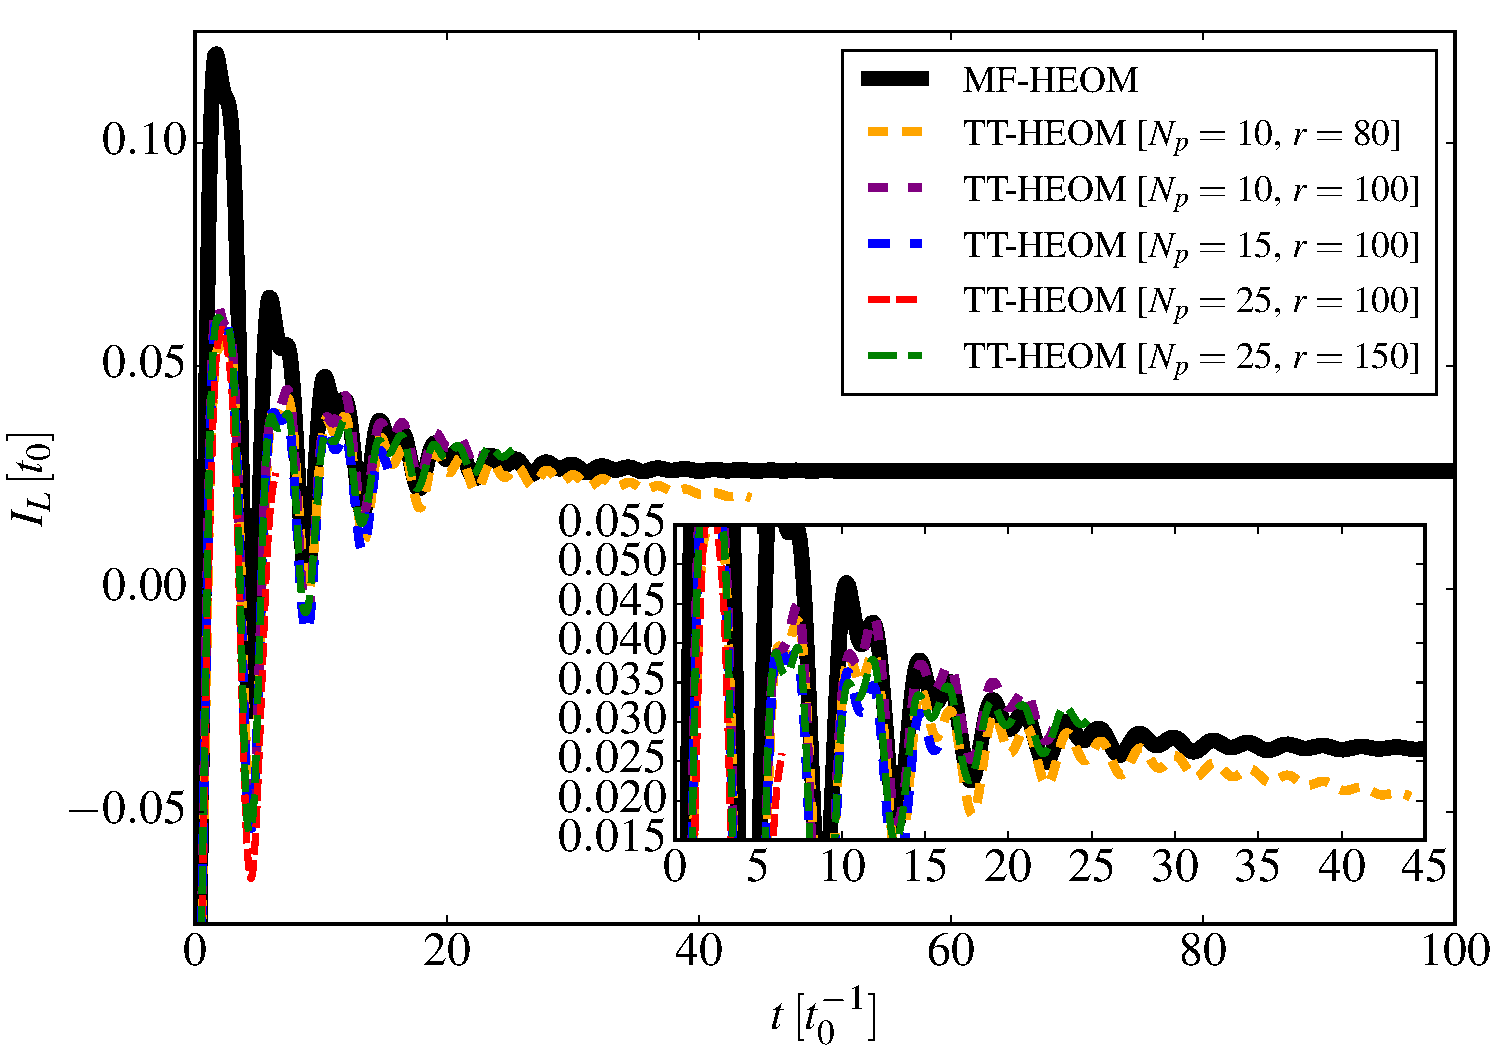
\includegraphics[width=0.65\textwidth]{../report_3/figs/Comparison_TTHEOM_TDVP_ED_hop+onsite+SOC_V10.pdf}
	\caption{Time-dependent current from the left lead into the system for a tight-binding model. Comparison of MF-HEOM with TT-HEOM for various number of Pad\'{e} poles $N_p$ and ranks.}
\end{figure}
\newpage
\section{Properties of the non-vibrating molecule}
\subsection{Current-voltage characteristics}
\begin{figure}[!h]
	\centering
	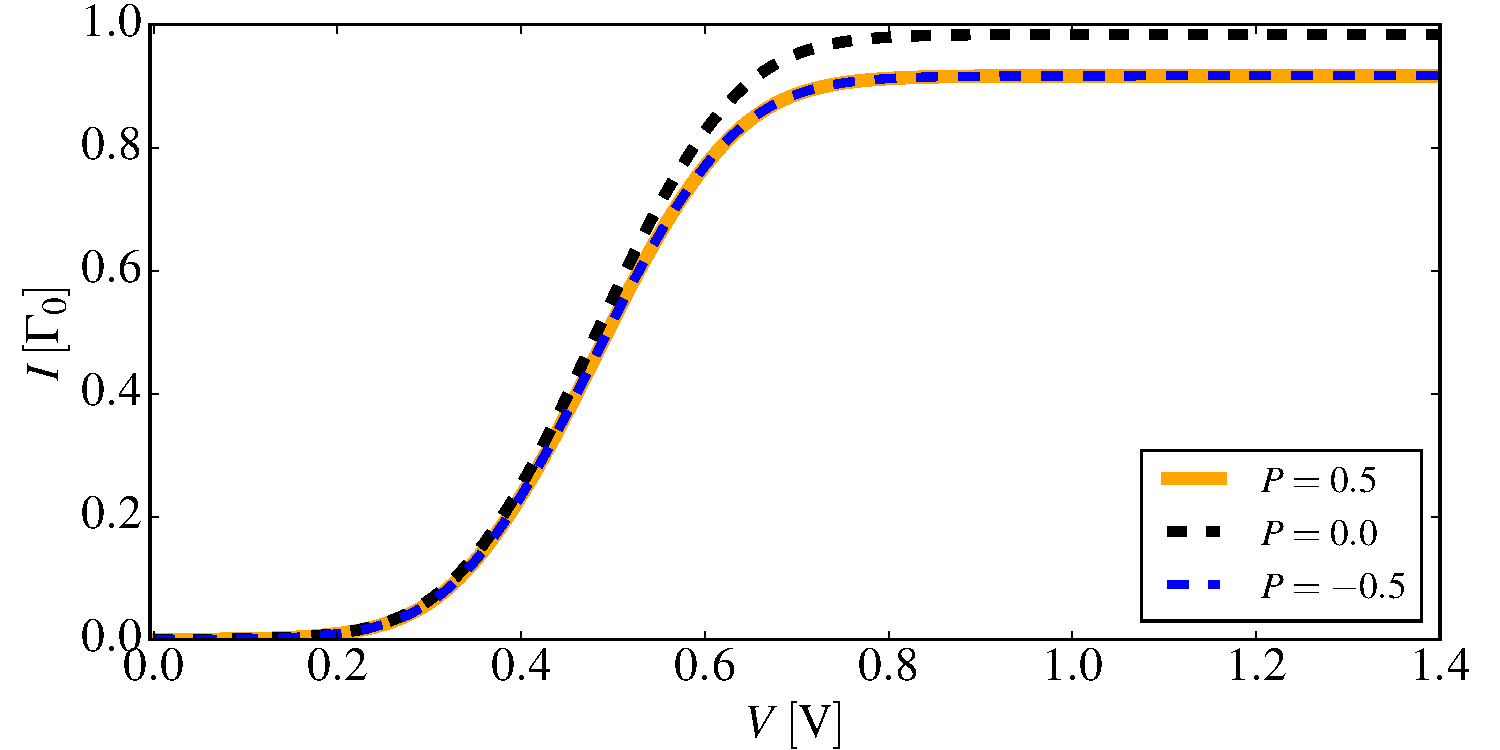
\includegraphics[width=0.65\textwidth]{figs/LB_1x3.pdf}
	\caption{Current-voltage characteristics for $\mathbb{M}=1\times 3$ and parameters as in the main text.}\label{fig:IV_1x3}
\end{figure}
\begin{figure}[!h]
	\centering
	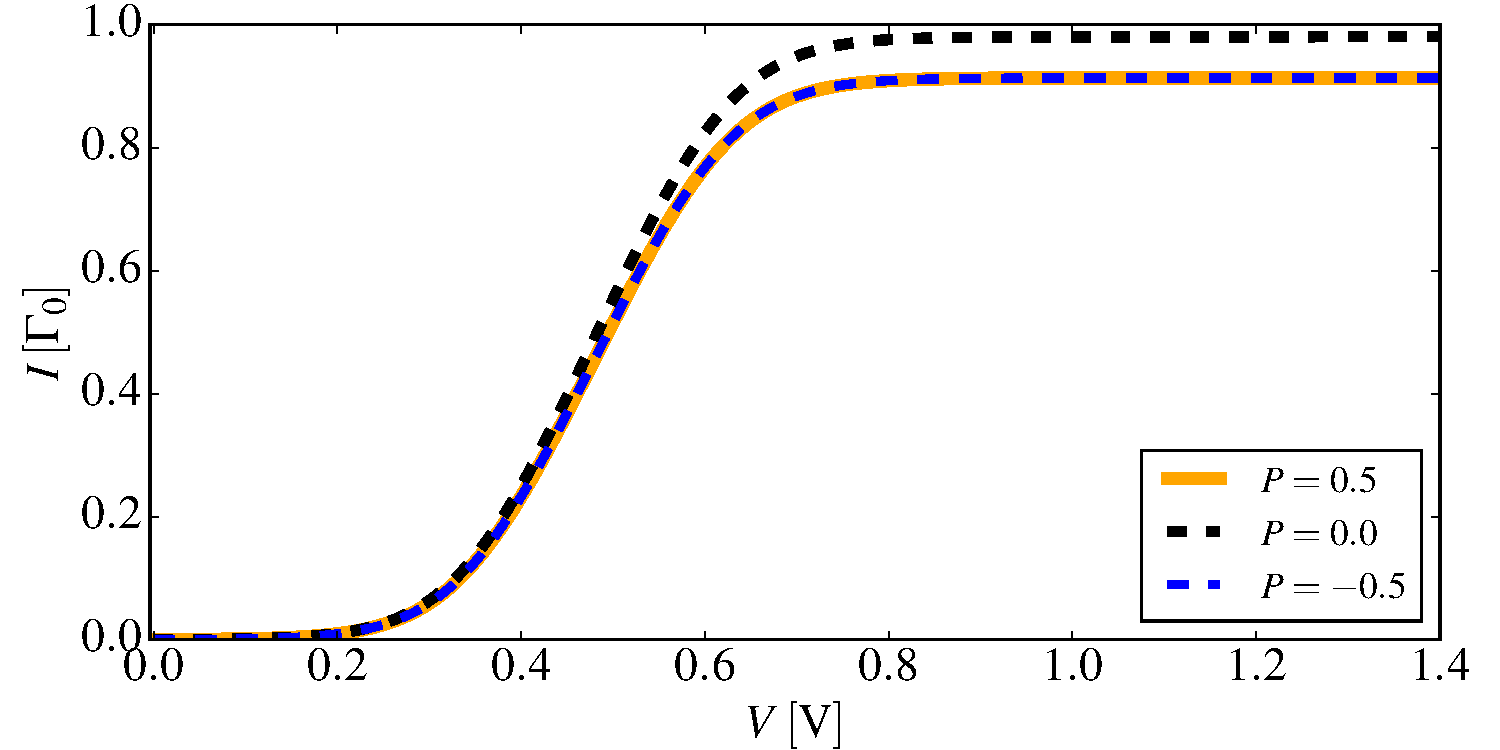
\includegraphics[width=0.65\textwidth]{figs/LB_4x3.pdf}
	\caption{Current-voltage characteristics for $\mathbb{M}=4\times 3$ and parameters as in the main text.}\label{fig:IV_4x3}
\end{figure}
The relative energies of the leads chemical potential and the bare electronic levels of the molecule are shown in \cref{fig:Schematic_Energy_levels}
\begin{figure}[!h]
	\centering
	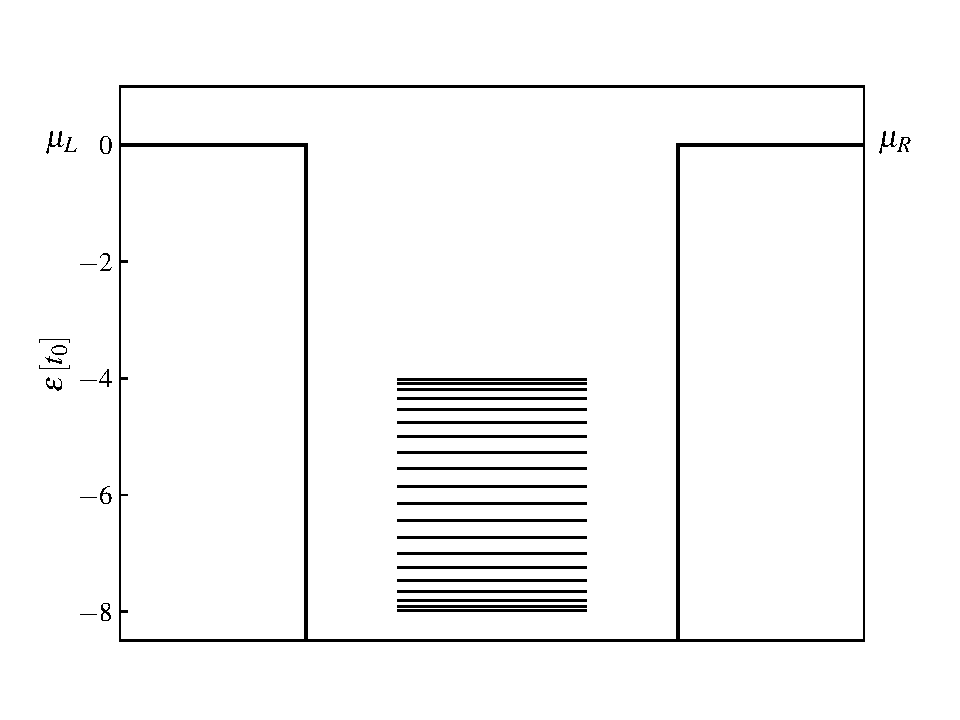
\includegraphics[width=0.55\textwidth]{../report_3/figs/Spectrum_leads.pdf}
	\caption{Schematic energy diagram of the Fransson model coupled to leads at $V=0$.}\label{fig:Schematic_Energy_levels}
\end{figure}\\
\subsection{Stationary electronic lattice occupation}\label{sec:Stationary_el_lat_occ}
\begin{figure}[!h]
	\centering
	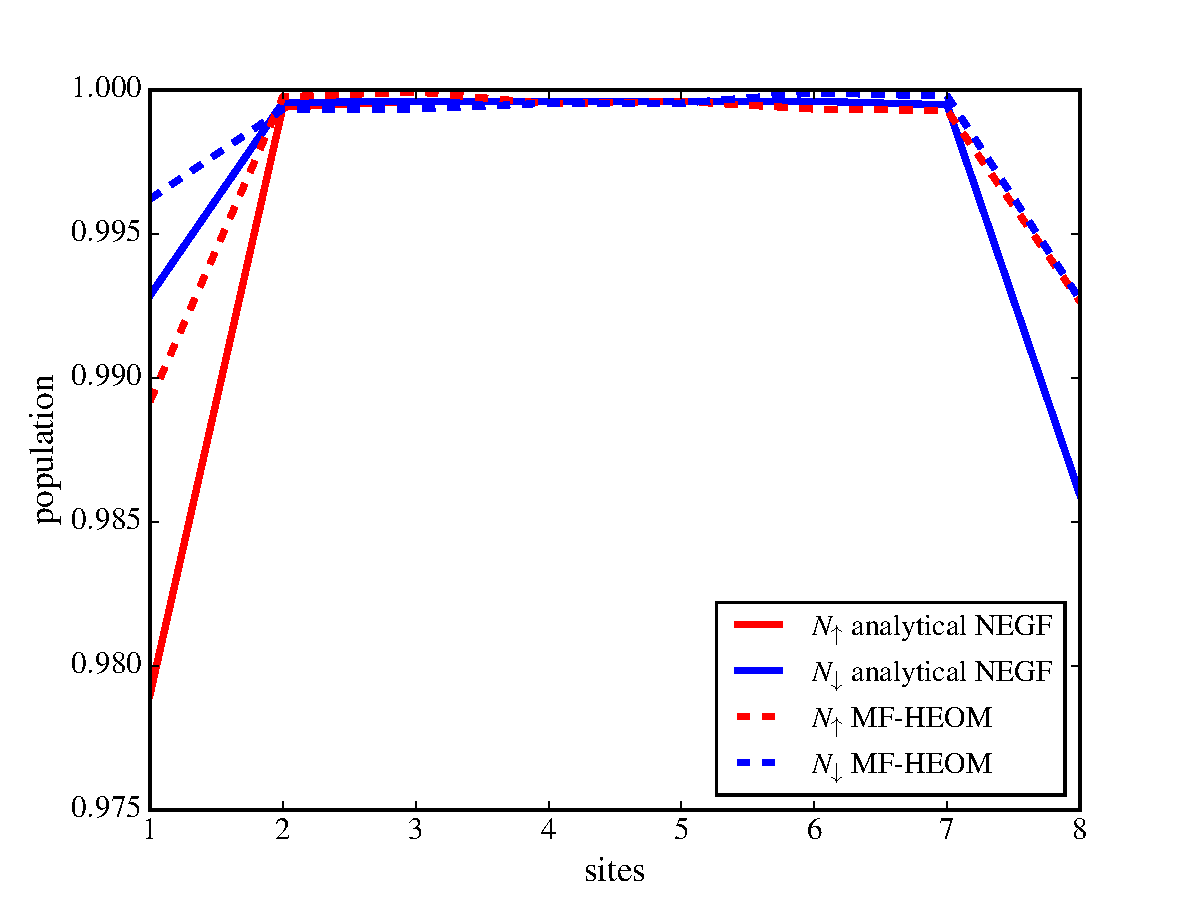
\includegraphics[width=0.75\textwidth]{figs/Comparison_populations_V0.pdf}
	\caption{Comparison of spin-dependent populations for $V=0$ from analytical NEGF expression (full lines) and numerically obtained population at $t=\SI{1.72}{\pico\second}$ (MF-HEOM, dashed lines).}\label{fig:Comp_NEGF_MF-HEOM_pops}
\end{figure}
\subsection{Population dynamics}
To understand the discrepancy between the equilibrium populations in the NEGF and HEOM approaches, we investigate population dynamics in the following. \Cref{fig:MF_2x4_PopDyn_noPh} shows the dynamics of population of spin-up and spin-down electrons on all sites of a $\mathbb{M}=2\times 4$ molecule. Over the time-interval investigated here, the populations do not reach a stationary value. Related to non-stationary populations are so-called equilibrium currents flowing between the leads and the molecule, which are shown in \cref{fig:MF_2x4_CurDyn_noPh} (black line).
\begin{figure}[!h]
	\centering
	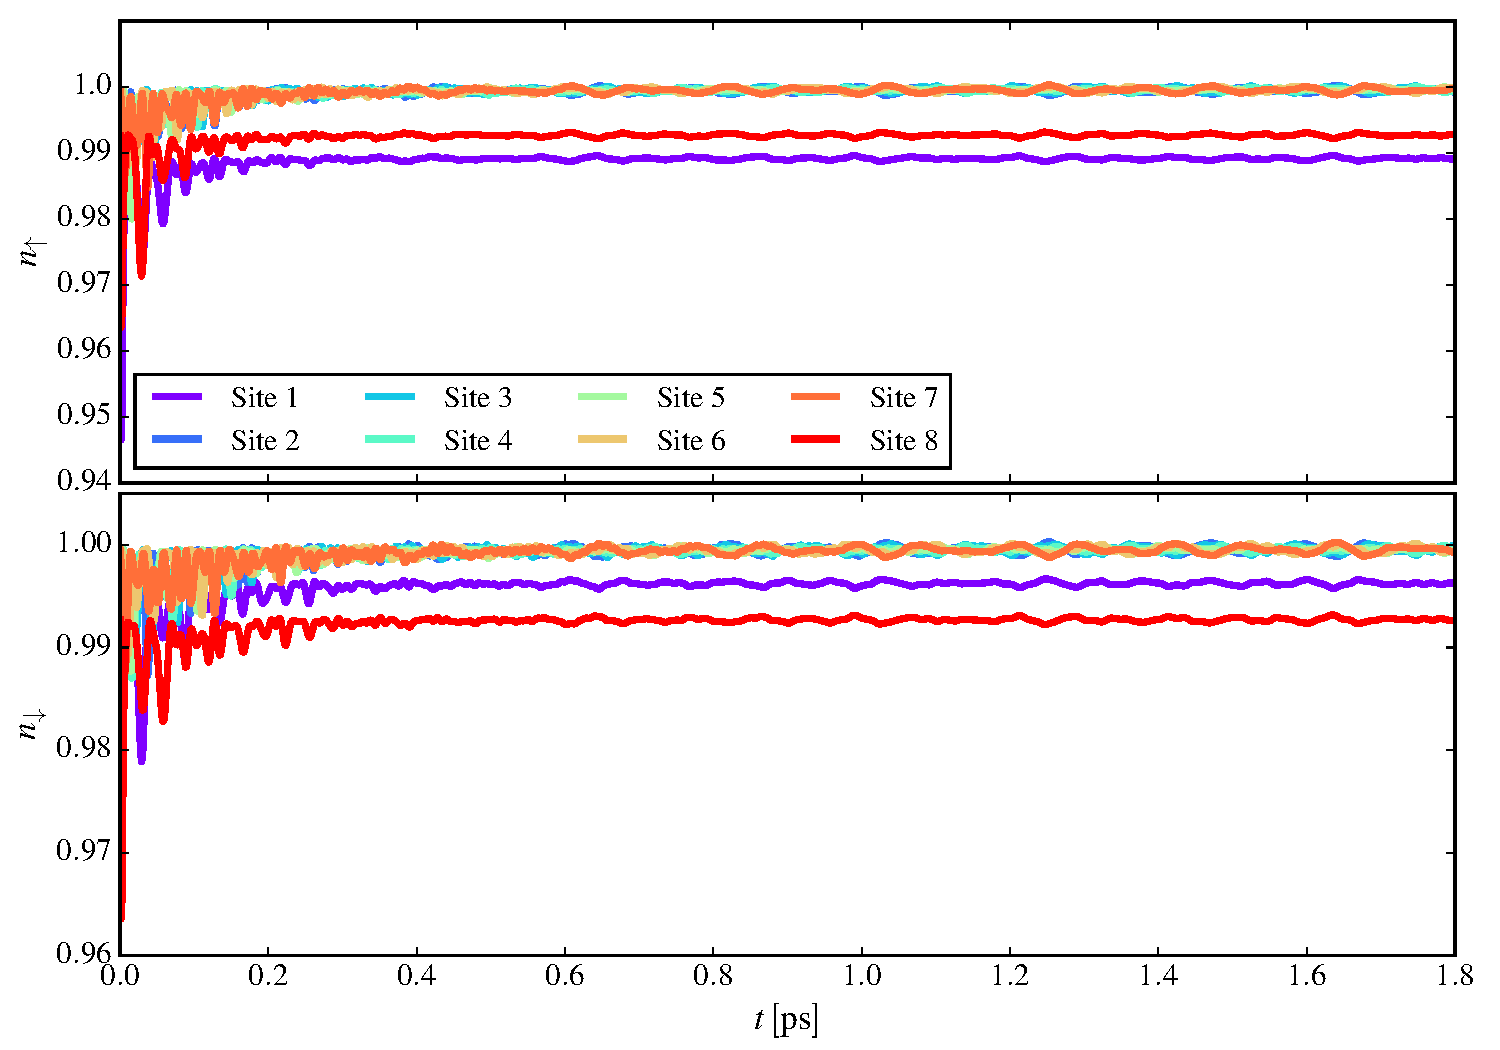
\includegraphics[width=0.99\textwidth]{figs/MF_noPh_2x4_population_dynamics_V0.pdf}
	\caption{Population dynamics of spin up (upper panel) and spin down (lower panel) electrons for $V=0$, $P=0.5$ and $\mathbb{M}=2\times 4$.}\label{fig:MF_2x4_PopDyn_noPh}
\end{figure}
\begin{figure}[!h]
	\centering
	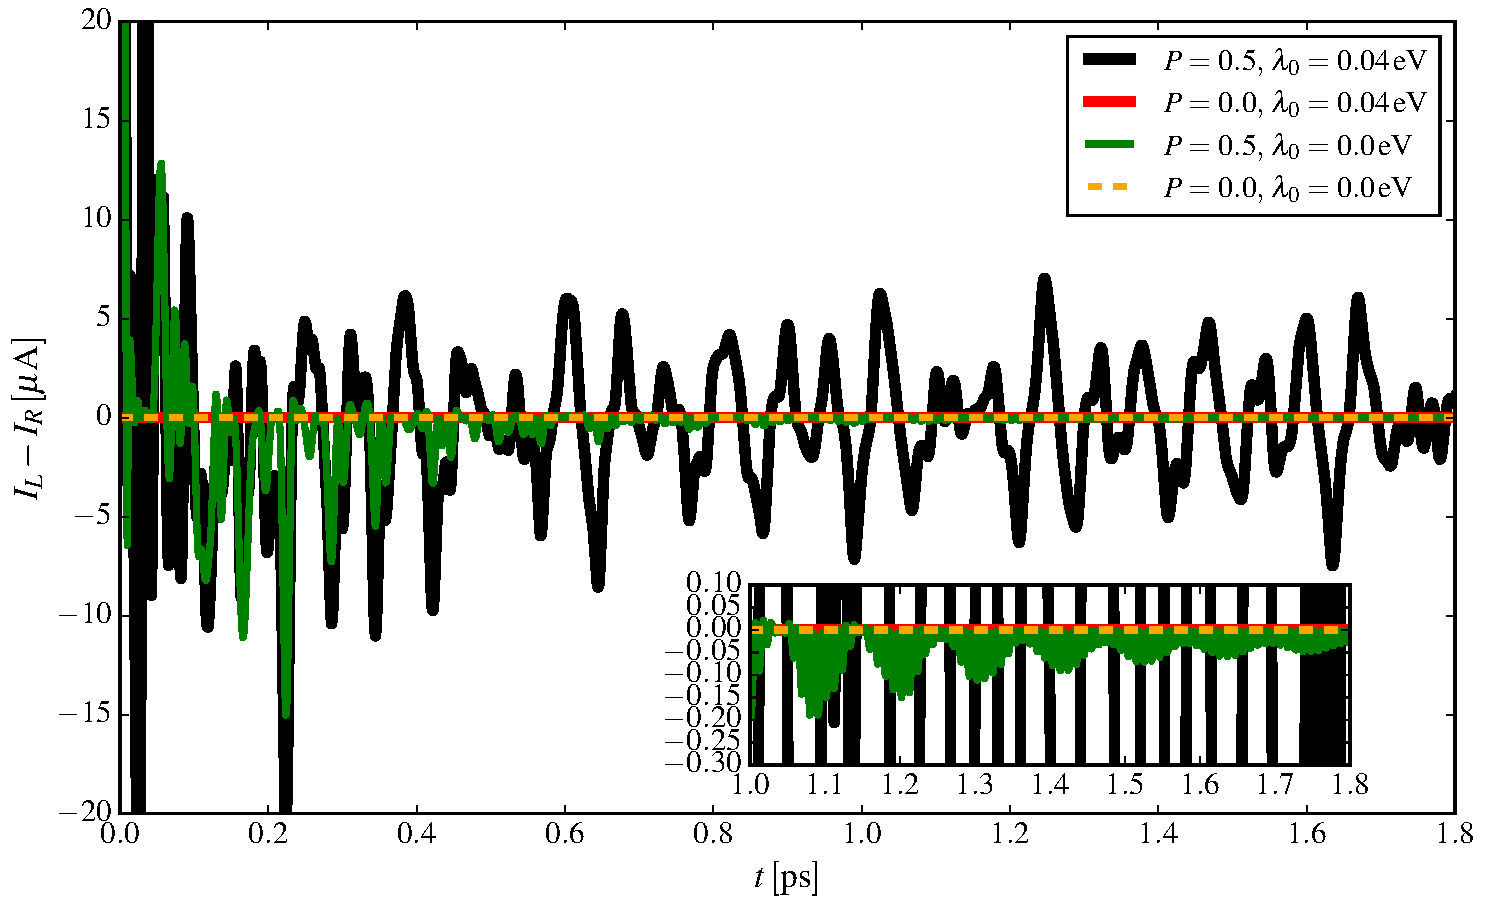
\includegraphics[width=0.99\textwidth]{figs/MF_noPh_2x4_current_dynamics_V0.pdf}
	\caption{Comparison of current dynamics for $V=0$ and $\mathbb{M}=2\times 4$ for $P=0.0,0.5$ and $\lambda_0=\SI{0.0}{\electronvolt},\SI{0.04}{\electronvolt}$.}\label{fig:MF_2x4_CurDyn_noPh}
\end{figure}\\
\Cref{fig:MF_2x4_CurDyn_noPh} compares the case where the left lead is spin-polarized and the SOC in the molecule is $\lambda_0=\SI{0.04}{\electronvolt}$ with the case of a molecule with SOC but spin-unpolarized left lead (red line), and the cases of a molecule without SOC with $P=0.5$ (green line) and $P=0.0$ (orange line). 
Even in the absence of SOC but for a spin-polarized lead, the current does not reach a steady state in the time-interval considered here. Thus, solely identifying SOC as the reason for equilibrium currents is suggestive, but one has to take into account also the spin-polarization of the lead.
This comparison suggests that the cause of these equilibrium currents is the interplay between the spin-orbit interaction in the molecule and the spin-polarization in the left lead.
\Cref{fig:MF_2x4_PopDyn_noPh_comp_Lambda}  shows the population on site 1 for $\lambda_0 = \SI{0.04}{\electronvolt}$ and $\lambda_0 = \SI{0.0}{\electronvolt}$. While the population in the molecule without SOC reaches a stationary value, the one with SOC does not.
\begin{figure}[!h]
	\centering
	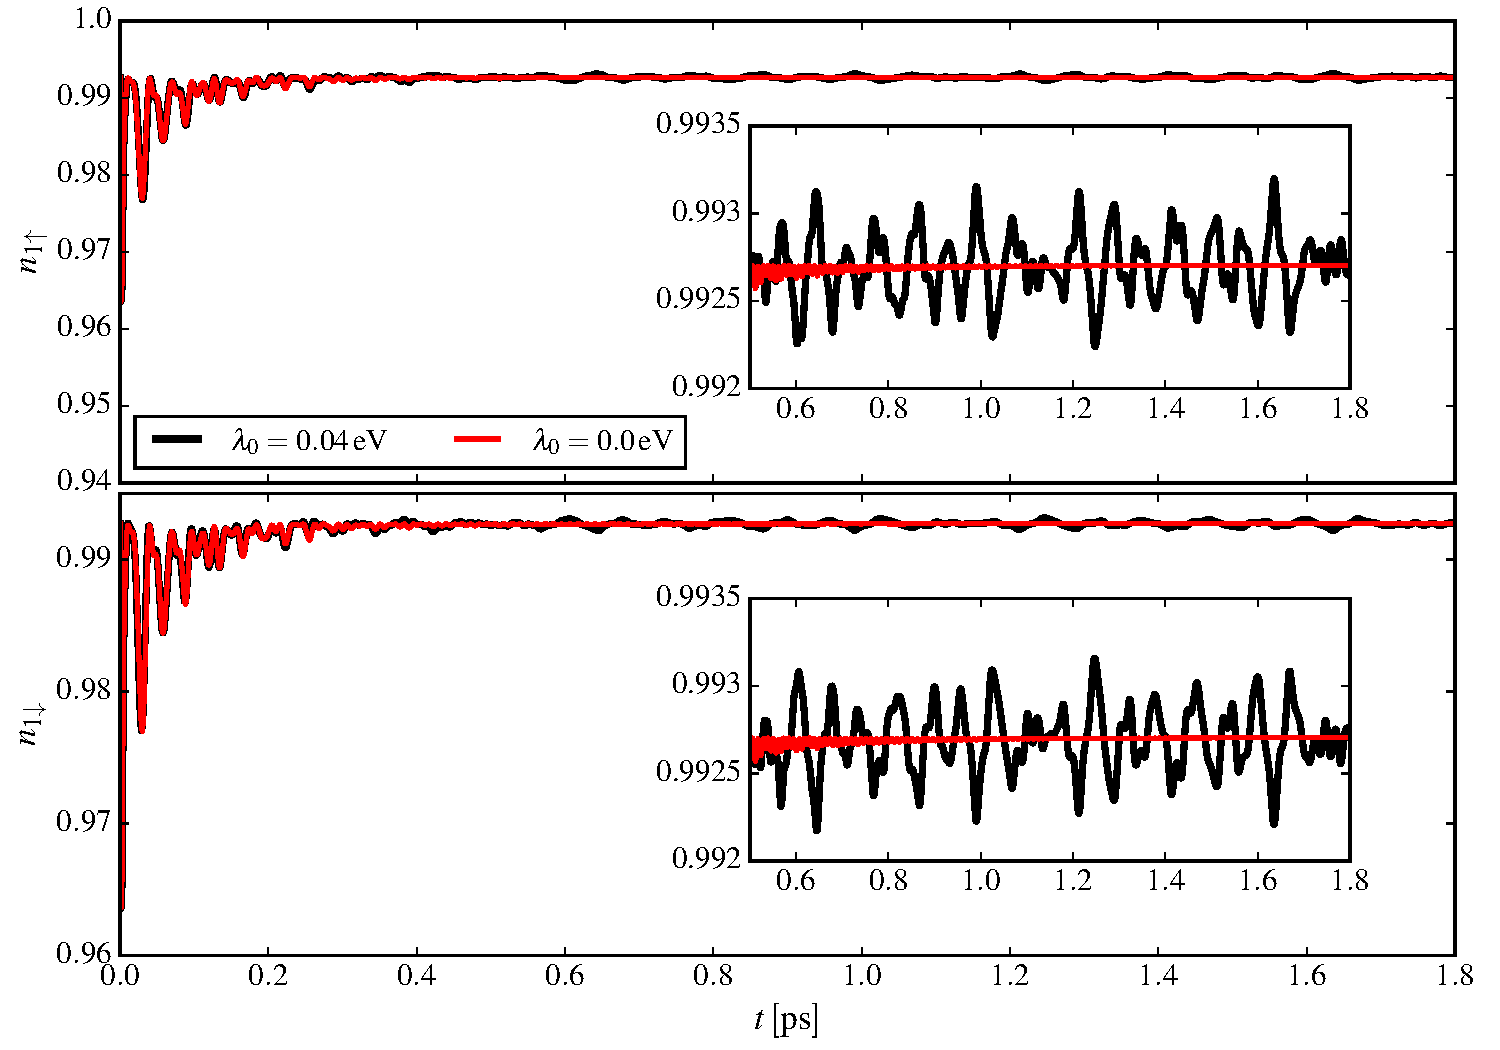
\includegraphics[width=0.99\textwidth]{figs/MF_noPh_2x4_population_dynamics_V0_P0_LambdaVar.pdf}
	\caption{Equilibrium population dynamics on site 1 for  $\mathbb{M}=2\times 4$ and $P=0$.}\label{fig:MF_2x4_PopDyn_noPh_comp_Lambda}
\end{figure}


\section{Ehrenfest approach: Tests of implementation}
\subsection{Reduction to classical MD for zero electron-phonon coupling}
For vanishing electron-phonon coupling, the nuclear dynamics reduces to a purely molecular dynamics integration. 
Then, the Hamiltonian reduces to 
\begin{equation}
	H = \sum_i \frac{\omega_i^2}{2}\left( X_i^2 + \frac{P_i^2}{w_i^2}\right) + H_\mathrm{el}\label{eq:TotalHamiltonian}
\end{equation}
where $H_\mathrm{el}$ is the purely electronic part of the total Hamiltonian. Since the vibrational modes are not coupled among each other, for the following analysis a single mode only is considered.
\begin{figure}[!h]
	\centering
	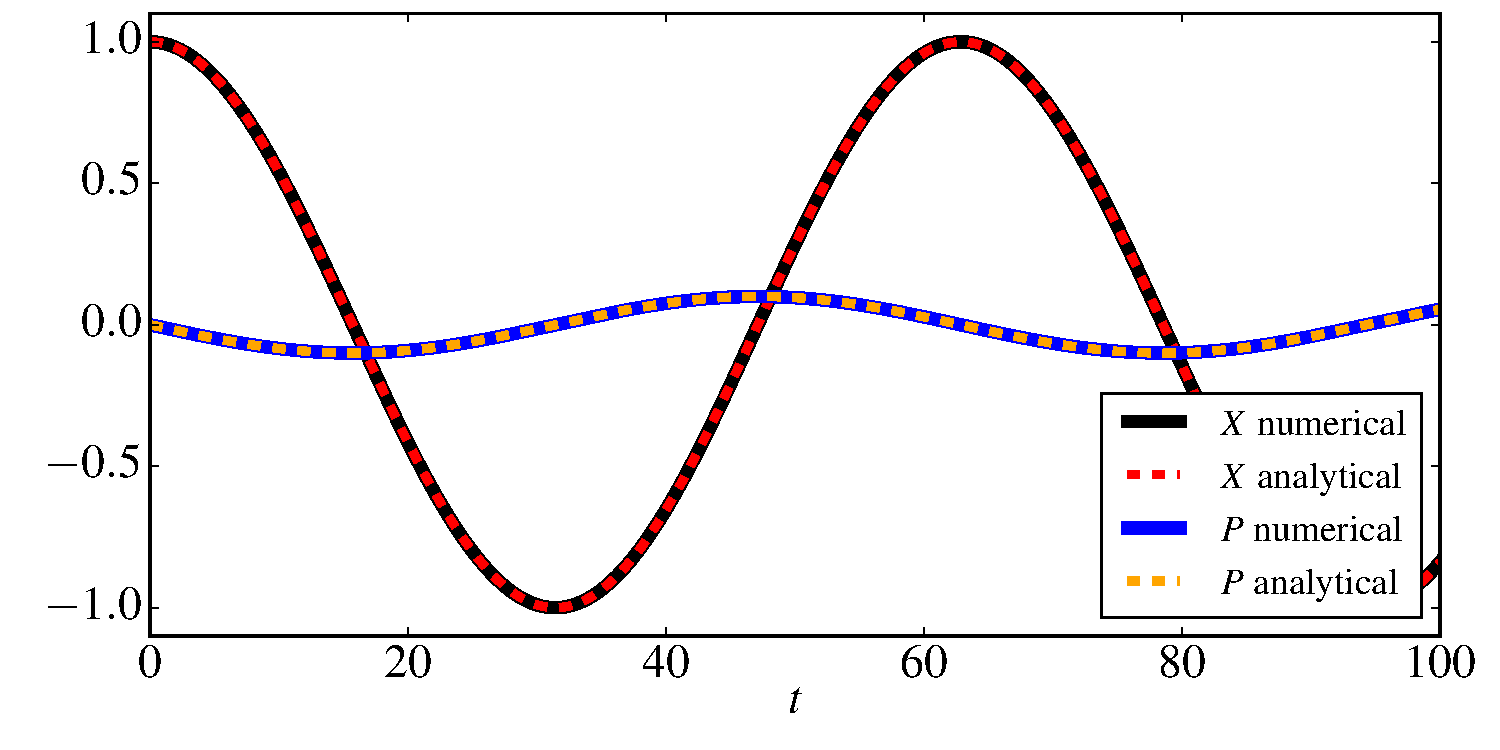
\includegraphics[width=0.7\textwidth]{figs/Decoupled_vibrational_dynamics.pdf}
	\caption{Numerical $X$, $P$ (black, blue line) and analytical functions (\cref{eq:AnalyticalVib1,eq:AnalyticalVib2}, dashed lines) for $\omega = 0.1$.}\label{fig:Comparison_Vib_Analytical}
\end{figure}\\
Then the Hamilton's equation of motion for vibrational coordinates and momenta read
\begin{align}
	\frac{\dif X}{\dif t} &= \frac{\partial H}{\partial P} =P\\
	\frac{\dif P}{\dif t} &= -\frac{\partial H}{\partial X} = -\omega^2 X\\
	X(0) &= X_0, P(0) = P_0
\end{align}
the solution of which can be found analytically as
\begin{align}
	X(t) &=  A\exP{i\omega t} +B\exP{-i\omega t} ,\label{eq:AnalyticalVib1}\\
	P(t) &=  i\omega (A\exP{i\omega t} -B\exP{-i\omega t}),\label{eq:AnalyticalVib2}
\end{align}
with $A = \frac{X_0}{2}+\frac{P_0}{2i\omega}$ and $B  = A^*$.
For the numerical comparison, $X_0 = 1$ and $P_0 = 0$ have been chosen. The numerical integration agrees with the analytical results, as shown in \cref{fig:Comparison_Vib_Analytical}.
%\subsection{Check of implementation of coupled dynamics}
%To check if the coupled electron-vibrational dynamics is implemented correctly, we consider a double dot with only a Peierls term in the electronic Hamiltonian
%\begin{equation}
%	H_\mathrm{el}(t) = -\sqrt{2\omega_0}t_1 X(t) (c_1^\dagger c_2^\pdagger +\mathrm{h.c.})\label{eq:PeierlsDoubleDot}
%\end{equation}
%in \cref{eq:TotalHamiltonian} coupled to two leads with level-width function $\bm{\Gamma}$. For $V=0$, the purely electronic dynamics for the reduced density matrix
%\begin{equation}
%	\frac{\dif}{\dif t}\bm{\rho}(t) = -i[\vec{H}^\mathrm{eff},\bm{\rho}]
%\end{equation}
%under the effective Hamiltonian matrix
%\begin{equation}
%	\vec{H}^\mathrm{eff} = \vec{H}_\mathrm{el} - \frac{i}{2}\bm{\Gamma}
%\end{equation}  
%agrees with dynamics obtained within the MF-HEOM. \Cref{fig:Comparison_NH_MFHEOM} shows a comparison of population dynamics in the single-site tight-binding model for the parameters $\varepsilon_0 = 0$, $\Gamma_L=\Gamma_R= \frac{t_0}{4}$, $n(0)=1$ with perfect agreement.
%\begin{figure}[!h]
%	\centering
%	\includegraphics[width=0.9\textwidth]{figs/Comparison_NH_HEOM_noPh.pdf}
%	\caption{Population dynamics within the MF-HEOM (black solid line) and the Liouville-von Neumann equation under the non-hermitian effective Hamiltonian $\vec{H}^\mathrm{eff} = \vec{H}_\mathrm{el}-\frac{i}{2}\bm{\Gamma}$ (red dashed line). }\label{fig:Comparison_NH_MFHEOM}
%\end{figure}\\
%Now turning to the case with electron-vibrational coupling in the form of \cref{eq:PeierlsDoubleDot}. With $t_1 = 0.2$, $\omega_0 = 0.1$, and $\Gamma_L=\Gamma_R=0$  
\subsection{Initial distribution of vibrational phase space coordinates}
As in the usual multi-trajectory Ehrenfest methodology, the initial vibrational phase space coordinates are sampled from the Boltzmann distribution for a harmonic oscillator in its ground state
\begin{equation}
	\rho(\{X\},\{P\}) = \prod_j \frac{\alpha_j}{\pi} \exp\left[-\frac{\alpha_j}{\omega_j} \left(P_j^2+\omega_j^2X_j^2\right)\right],\label{eq:Boltzmann_probabilityDist}
\end{equation} 
with $\alpha_j = \tanh(\frac{1}{2}\beta \omega_j)$.
In the numerical calculation, pseudo-random numbers are sampled from this distribution at the initial time. \Cref{fig:Comparison_Pdist_analytical_numerical} shows a comparison of the analytical probability density distribution with a histogram of numbers randomly sampled from this distribution.
\begin{figure}[!h]
	\centering
	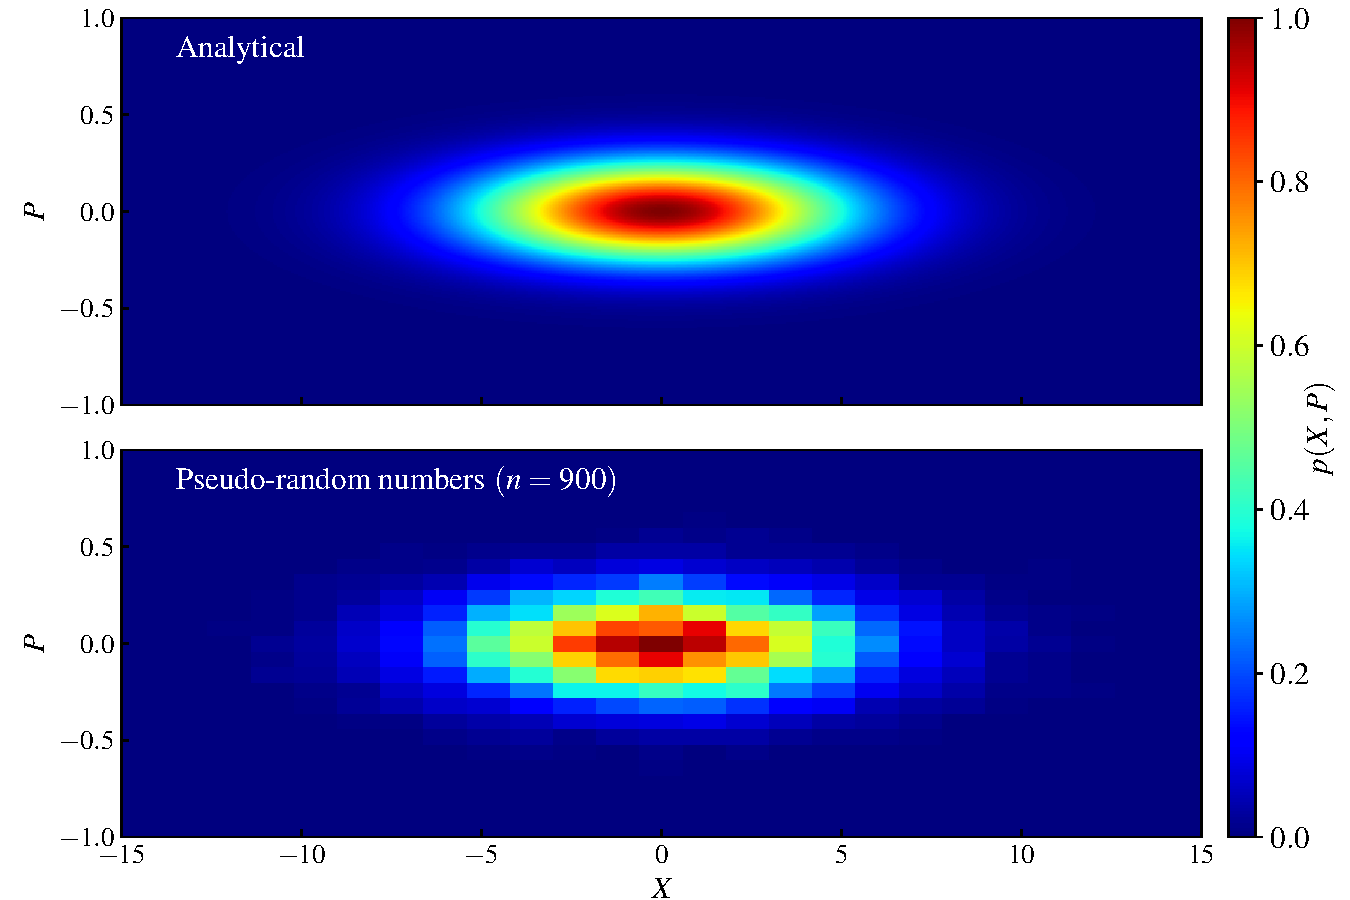
\includegraphics[width=0.95\textwidth]{../report_3/figs/Comparison_Pdist_analytical_numerical.pdf}
	\caption{Comparison of analytical harmonic oscillator Boltzmann probability density distribution ($\omega = 0.05$, $\beta = 40$) with pseudo-random numbers sampled from the same distribution (samplesize $n=900$).}\label{fig:Comparison_Pdist_analytical_numerical}
\end{figure}\\
\section{Existence of a unique steady-state}
\subsection{Vibrational steady-state: Adiabatic approximation}
{\color{red}{Michael mentioned that there is no steady state because EOM is simply shifted Harmonic Oscillator. Clarify.}}
The classical dynamical system can be represented by a vector $\bm{\xi} = (X_1,P_1,\dots,X_n,P_n)$ such that the classical equation of motion is 
\begin{equation}
	\frac{\dif }{\dif t}\bm{\xi} = \mathcal{M}\bm{\xi} + \vec{b}(\langle\rho\rangle),
\end{equation}
where 
\begin{equation}
	\mathcal{M} = \begin{pmatrix}
		0 & \omega_0 & 0 & 0 &\dots & 0\\
		-\omega_0^2 & 0 & 0 &  0& \dots & 0\\
		0 & 0 & 0 & \omega_0 & \dots & 0\\
		0 & 0 & -\omega_0^2 & 0 & \dots & 0\\
		\vdots &   &  &\ddots  & &\vdots\\
		0 & \dots & & &  &0
	\end{pmatrix}
\end{equation}
and 
\begin{equation}
	\vec{b}(\langle \bm{\rho}\rangle) = \begin{pmatrix}
		0 \\
		-\tr{\bm{\rho} \partial_{X_1}\vec{H}_\mathrm{el-ph}}\\
		0\\
		\vdots\\
		0 \\
		-\tr{\bm{\rho} \partial_{X_{N-1}}\vec{H}_\mathrm{el-ph}}\\
	\end{pmatrix}.
\end{equation}
The steady-state is then given by
\begin{equation}
	\bm{\xi}_\mathrm{ss} = -\mathcal{M}^{-1}\vec{b}.
\end{equation}
For example, for $\mathbb{M}=1\times 2$, there is a single bond only, and therefore only a single vibrational mode. 
The steady-state can be read off directly from the equation of motion
\begin{equation}
	\bm{\xi}_\mathrm{ss} = \frac{1}{\omega_0}\begin{pmatrix}
		\tr{\bm{\rho} \partial_{X}\vec{H}_\mathrm{el-ph}}\\
		0
	\end{pmatrix}.\label{eq:PhaseSpace_NESS}
\end{equation}
We conclude, that both electronic and vibrational systems, when treated independently, have a unique steady-state.
\subsection{Numerical investigation of steady-states in the coupled dynamical system}
{\color{red}{Investigate molecule with $\lambda_0=\lambda_1=\SI{0.0}{\electronvolt}$. Does current still oscillate? Draw connection to \cref{fig:MF_2x4_PopDyn_noPh}.}}
In this section we investigate numerically if a steady-state is reached in the coupled electron-vibrational Ehrenfest-dynamics for the open Fransson model (considering the same parameters as before with $P=0.5$). 
\begin{figure}[!h]
	\centering
	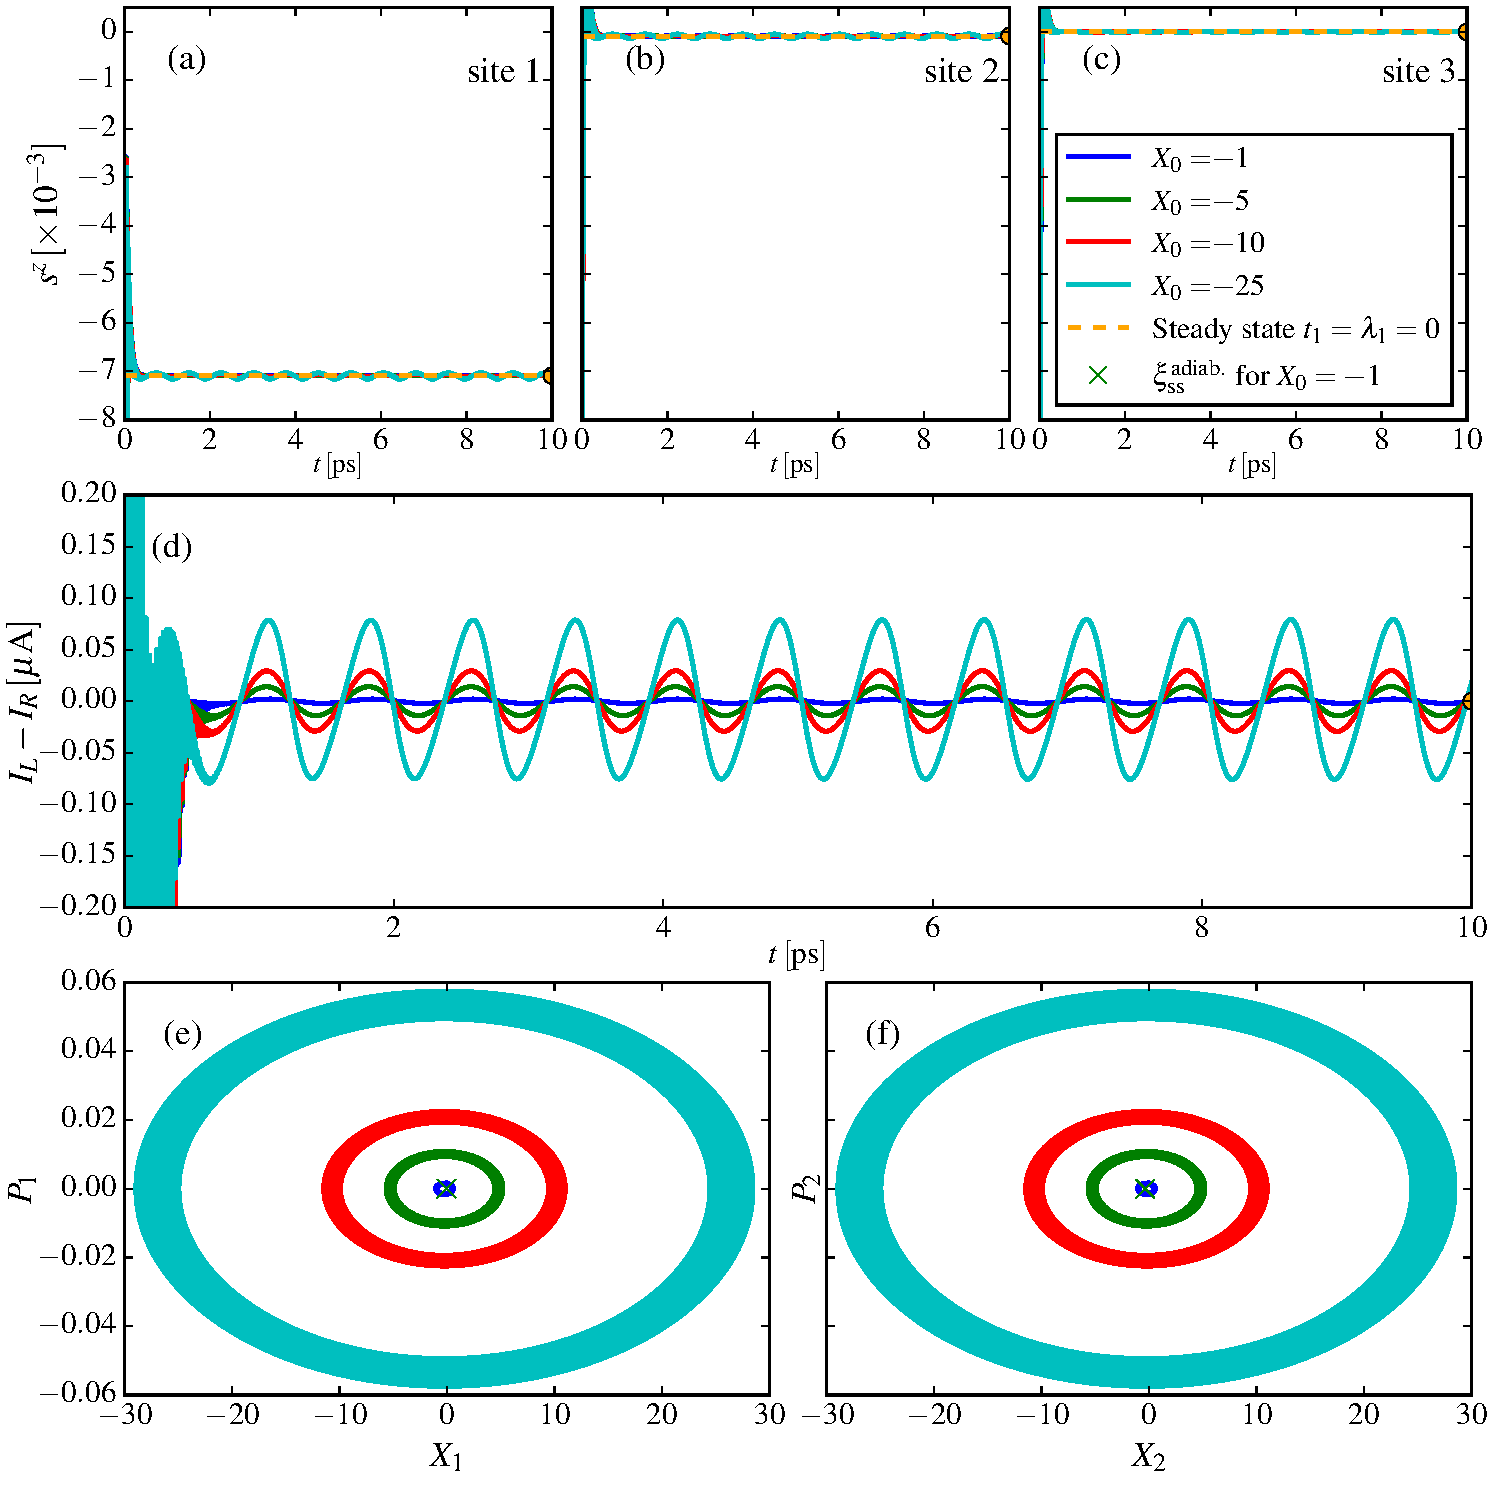
\includegraphics[width=0.94\textwidth]{figs/Pops_currents_phonons_1x3_V0.pdf}
	\caption{(a),(b) and (c) local spin polarization on sites 1,2, and 3, respectively. (d) Symmetrized current. (e) and (f) phase space trajectories of the two vibrational modes. Different lines show different initial conditions for the vibrational positions $X_0$. The dashed orange line shows quantities in the steady state for $t_1=\lambda_1 = 0$.}\label{fig:Pops_currents_phonons_1x3_V0}
\end{figure}\\
For this, the coupled quantum-classical HEOM equations of motion are solved where the initial vibrational coordinates are varied (and not sampled from the distribution given in \cref{eq:Boltzmann_probabilityDist}).

We start with the equilibrium case $V=0$. Shown in \cref{fig:Pops_currents_phonons_1x3_V0} (a), (b), and (c) are the local spin polarization $s_i^z = \tr{\rho_i \sigma^z}$ on sites $i=1,2,3$, in (d) the symmetrized current $I_L-I_R$, and the phase-space trajectory of phonons at the bond between site 1 and 2 (e) and at the bond between sites 2 and 3 (f). The different lines show initial conditions $X_0=-1,-5,-10,-25$ for both modes. The initial vibrational momenta are set to $P_1(0)=P_2(0)=0$ in all cases.
We further compare the local spin polarization and the current with the ones obtained for $t_1 = \lambda_1=0$ (orange dashed line). The green cross in (e) and (f) indicates the steady state phase space point under the adiabatic approximation
\begin{equation}
	\bm{\xi}^\mathrm{adiab.}_\mathrm{ss} = \bm{\xi}_\mathrm{ss} (\rho_\mathrm{ss}^\mathrm{FNA}),
\end{equation}
which is the steady-state solution given in \cref{eq:PhaseSpace_NESS} with the steady-state density matrix under the fixed nuclei approaximation, $\rho_\mathrm{ss}^\mathrm{FNA}$. The steady-state density matrix in the FNA is obtained by propagating the HEOM under the full Hamiltonian (for a given $X_0,P_0$) but without propagating the classical degrees of freedom. 

For an initial condition $X_0\neq 0$, the local spin polarization and the symmetrized current follow the vibrational oscillation.
There is a current from left to right when $X_1,X_2<0$ and from right to left when $X_1,X_2>0$.  
Within the time-interval considered here, the current does not reach a steady state. 
Instead, it reaches a limit cycle.
Averaged over time, however, the current is zero.
Note that the amplitudes of oscillation of the spin polarization and the current are rather small compared to their steady-state values.
Also, no damping of the vibrational modes is observed, and the oscillation is stable. 
An exception is the case for $X_0=0$. Here, the vibrational modes are already in their steady state from the beginning $t=0$ and show basically no dynamics. 
Simultaneously, the current reaches a steady state in this case. 
Another important point is that the steady-state phase space point under the adiabatic approximation $\bm{\xi}^\mathrm{adiab.}_\mathrm{ss}$ agrees well with the numerical steady-state. 
We now proceed with the same analysis to a moderate voltage $V=12$, shown in \cref{fig:Pops_currents_phonons_1x3_V12}.
\begin{figure}[!h]
	\centering
	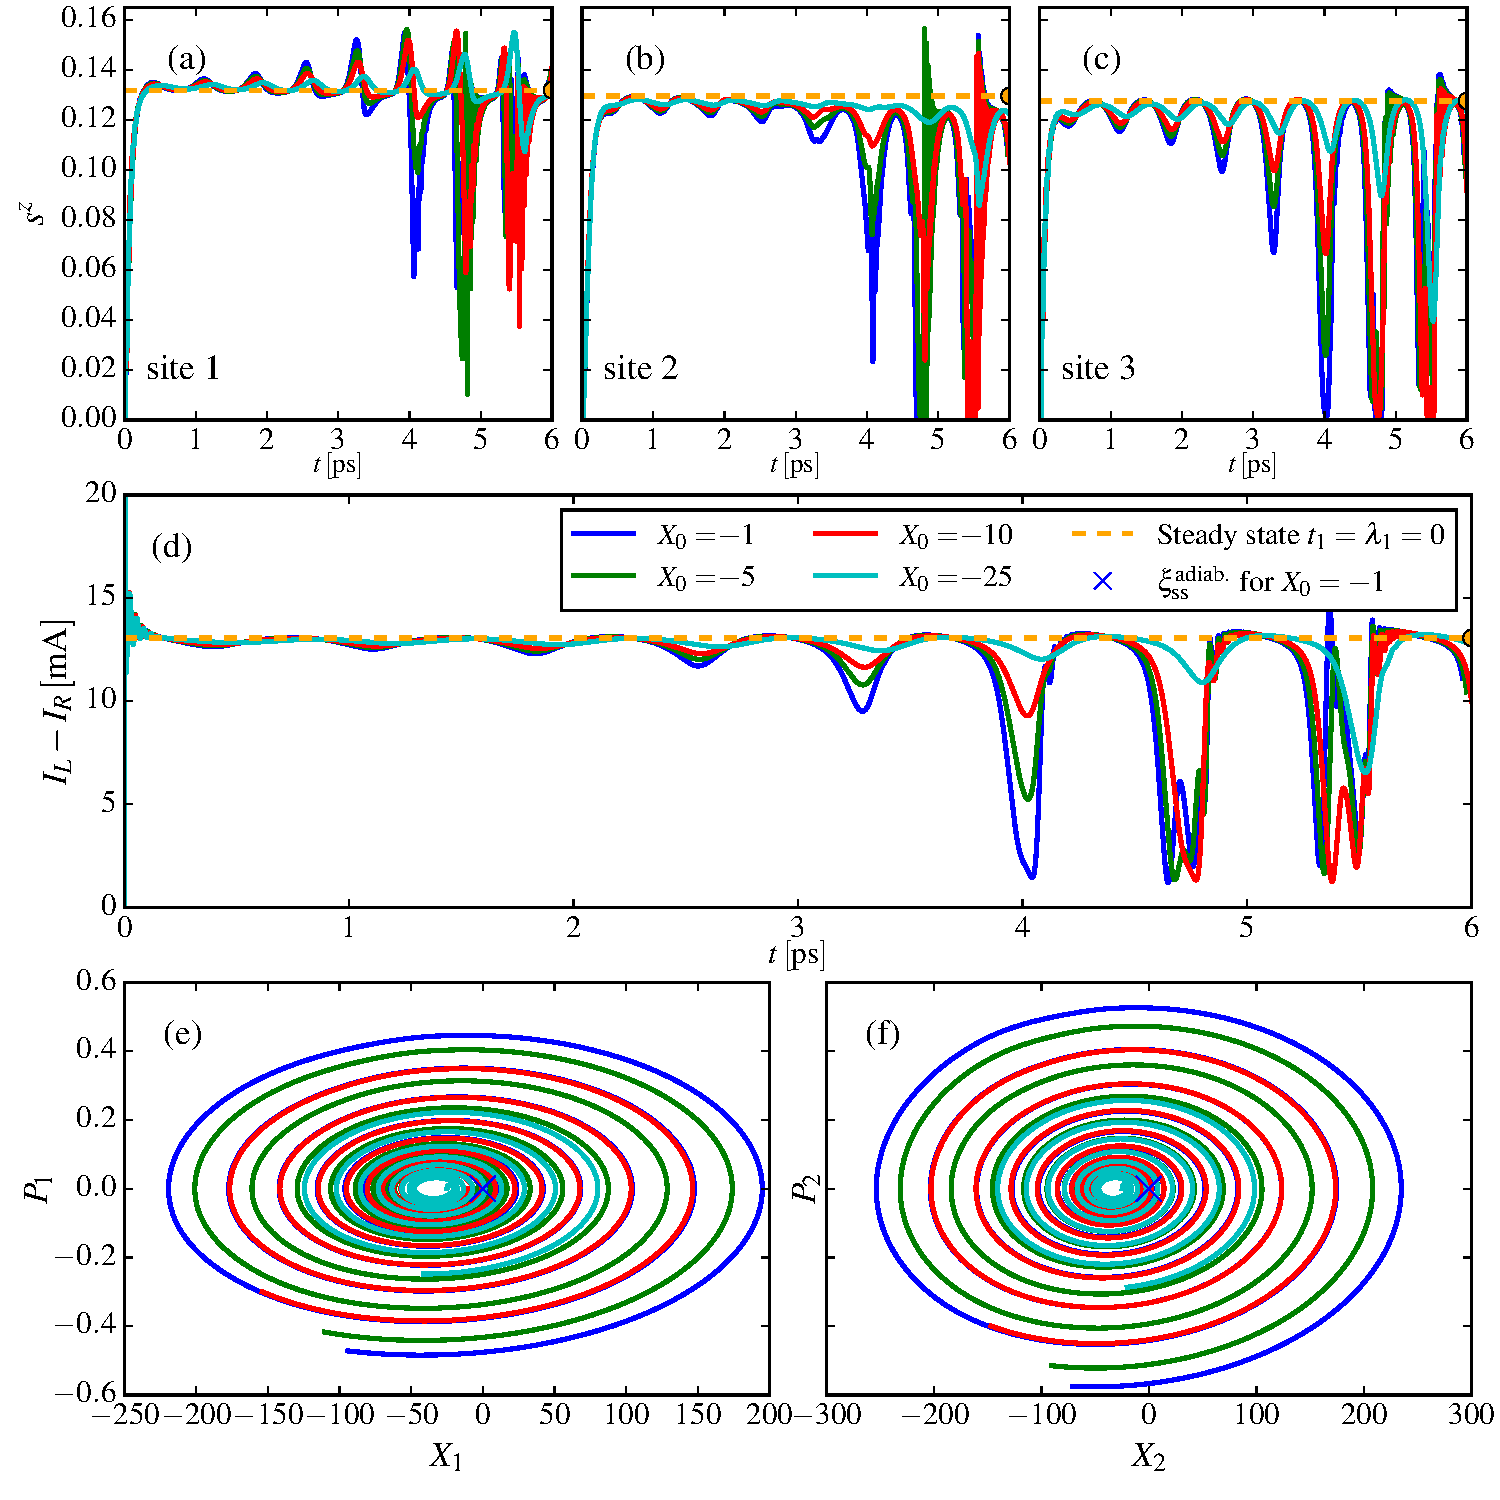
\includegraphics[width=0.94\textwidth]{figs/Pops_currents_phonons_1x3_V0.48.pdf}
	\caption{Same as \cref{fig:Pops_currents_phonons_1x3_V0} for $V=\SI{0.48}{V}$.}\label{fig:Pops_currents_phonons_1x3_V12}
\end{figure}\\
Beginning with the spin polarization, one can see that the time-dependence is not periodic anymore, unlike in the case $V=0$. On site 1, the spin polarization is for some time-interval even larger than the steady-state result obtained for $t_1=\lambda_1 = 0$. For later times and sufficiently large $X_0$, the spin polarization almost vanishes temporarily. On sites 2 and 3, this effect is observed for all investigated $X_0$, although the drop in spin polarization depends on $X_0$.
In contrast, the current is almost never larger than the steady-state current obtained for $t_1=\lambda_1=0$. The dynamics of the vibrational modes leads to a temporary reduction of the current.
The vibrational dynamics deviates significantly from the single harmonic-oscillator like phase-space portrait for $V=0$, covering larger parts of the phase space as energy from the electronic system is absorbed. 
In the time-interval considered here, the vibrational coordinates reach a limit cycle, which appears to be stable.
Also, the equilibrium of the vibrational position is shifted to $X\approx -10$. 
When $X_0$, however, is chosen carefully, the time-dependence of current and the populations can be reduced, such that a near-steady-state solution is found.
An interesting point is that the numerical steady-state phase-space point deviates strongly from $\bm{\xi}^\mathrm{adiab.}_\mathrm{ss}$.
We checked that the steady-state phase space point is voltage-dependent (but will not show any analysis on this). 
To conclude, the results have following implications (not in general, but only within the Ehrenfest-approach considered here):
\begin{itemize}
	\item Given an arbitrary $\bm{\xi}_0$, a steady-state may not exist (but a limit-cycle may exist).
	\item There exist $\bm{\xi}_0$, for which the time-dependence of long-time observables is small. (Speculation) When averaged over many trajectories normally distributed with means $\bm{\xi}_0$, a steady-state may be obtained as time-dependent contributions could cancel out.
	\item The $\bm{\xi}_0$ which are close to steady-state, depend on $V$ and may deviate from the null vector. (Speculation) Even when when trajectories are sampled from \cref{eq:Boltzmann_probabilityDist} and quantities are obtained from a weighted average, a steady-state may not be found for all voltages.
\end{itemize} 
\begin{itemize}
	\item Observation: $V=0$, current dynamics determined by SOC. When there is a voltage-induced current, dynamics is determined by $t_1$ (see MeanField\_v2\_weighting/Tests\_2x4).
	\item Phonons trap charge.
\end{itemize}
\newpage
\section{Multi-trajectory Ehrenfest dynamics approach to the Fransson model}
\subsection{Convergence with number of trajectories}
In the following, the parameters are the same as before: $t_0 = 1$, $\lambda_0 = t_0/40$, $t_1 = 0.1t_0$, $\lambda_1 = 0.1\lambda_0$, $\omega_0 = 0.05t_0$ $\Gamma_0 = t_0/4$ and $\beta = 40$.
Note, that in \cite{fransson2020vibrational}, a dimensionless coupling $t_1/\omega_0 = 10$ is used, whereas here we use $t_1/\omega_0 = 2$. Thus we are in a parameter regime which is much easier to converge.  
\Cref{fig:Current_convergence} shows the time-dependent symmetrized current $I_L(t)-I_R(t)$ for $V=18$ and $P=0.5$. Therein, gray faint lines are single trajectories, the red solid line is the weighted average for $n=100$ trajectories (weighted by the probability obtained from \cref{eq:Boltzmann_probabilityDist}) and the dashed orange line averaged over $n=1000$ trajectories. 
It has been checked, that the absolute normalized difference between averaged currents for $n=100$ and $n=1000$ is below $0.05\%$.  
\begin{figure}[!h]
	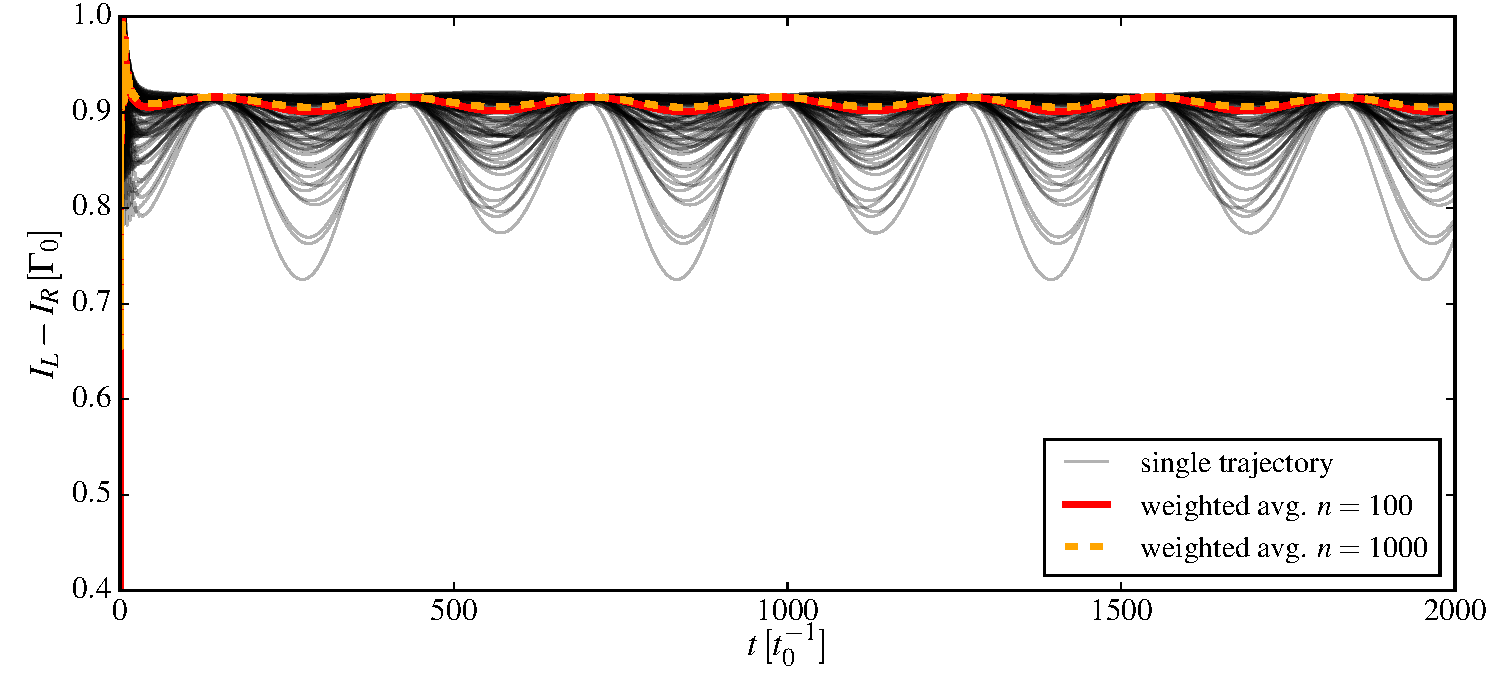
\includegraphics[width=0.8\textwidth]{../report_3/figs/Currents_1x3_Ehrenfest_noAvg_V18.pdf}
	\caption{Symmetrized time-dependent current for $P=0.5$ and $V=18.0$ for $\mathbb{M}=1\times 3$.}\label{fig:Current_convergence}
\end{figure}\\
However, for a smaller voltage, much more trajectories are necessary to converge the results. \Cref{fig:Current_V12_convergence} shows the weighted average of the symmetrized current for four different number of trajectories. The difference in current for $n=100$ and $n=1500$ is much larger compared to the case $V=18$ shown in \cref{fig:Current_convergence}.
\begin{figure}[!h]
	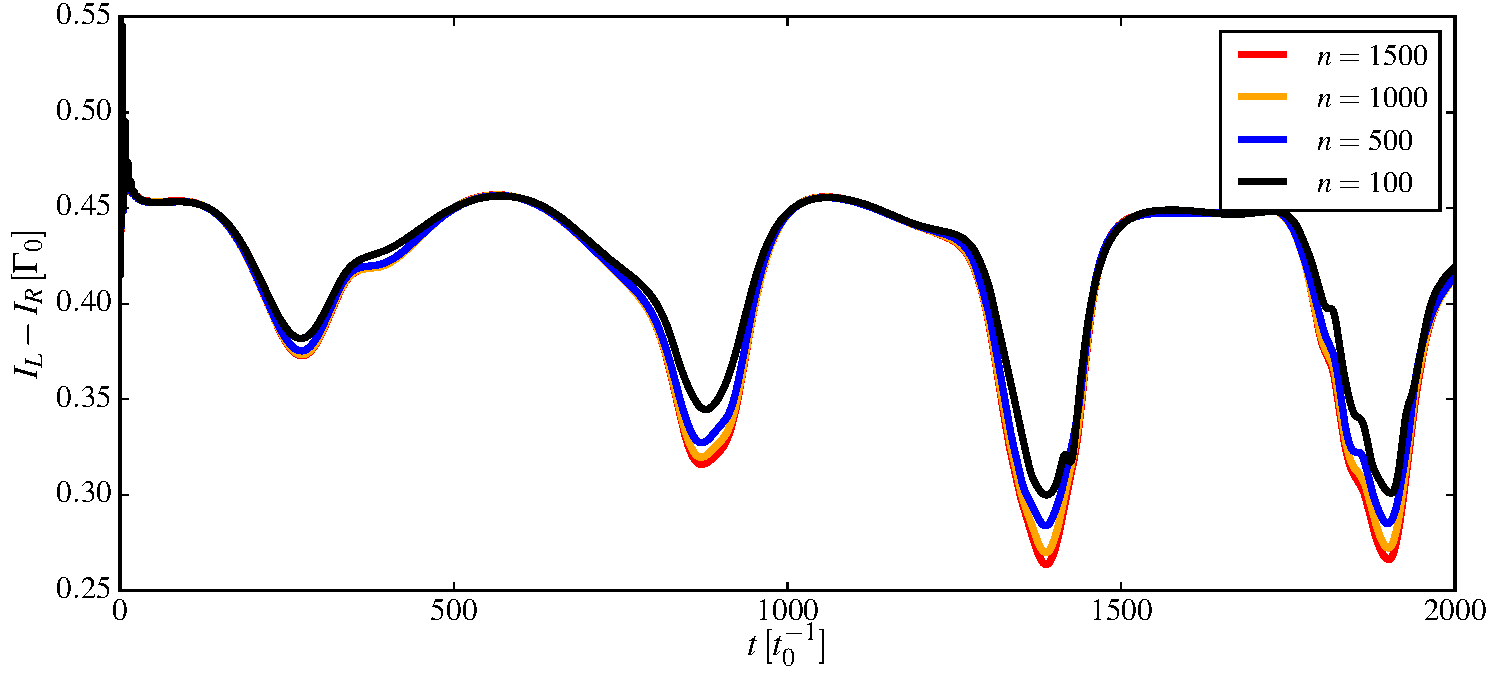
\includegraphics[width=0.8\textwidth]{../report_3/figs/Currents_1x3_Ehrenfest_V12.pdf}
	\caption{Symmetrized time-dependent current for $P=0.5$ and $V=12.0$ for $\mathbb{M}=1\times 3$.}\label{fig:Current_V12_convergence}
\end{figure}\\
It is apparent, that the no steady-state is reached in the time interval considered in the calculation. Rather a limit cycle is reached. These results confirm the third point given in the previous section. 
\subsection{Time-dependent vibrational phase space density}
\Cref{fig:TD_PSdensity} shows the time-evolution of the vibrational phase-space density for $t_0 = 1, t_1 = 0.1t_0, \lambda_0 = t_0/40, \lambda_1 = 0.1\lambda_0, \omega_0 = 0.05t_0, P = 0.5$, and $V=10t_0$ obtained for  $N_\mathrm{traj} = 900$. During time-evolution, the vibrational distribution deviates strongly from the initial equilibrium distribution.
\begin{figure}[!h]
	\centering
	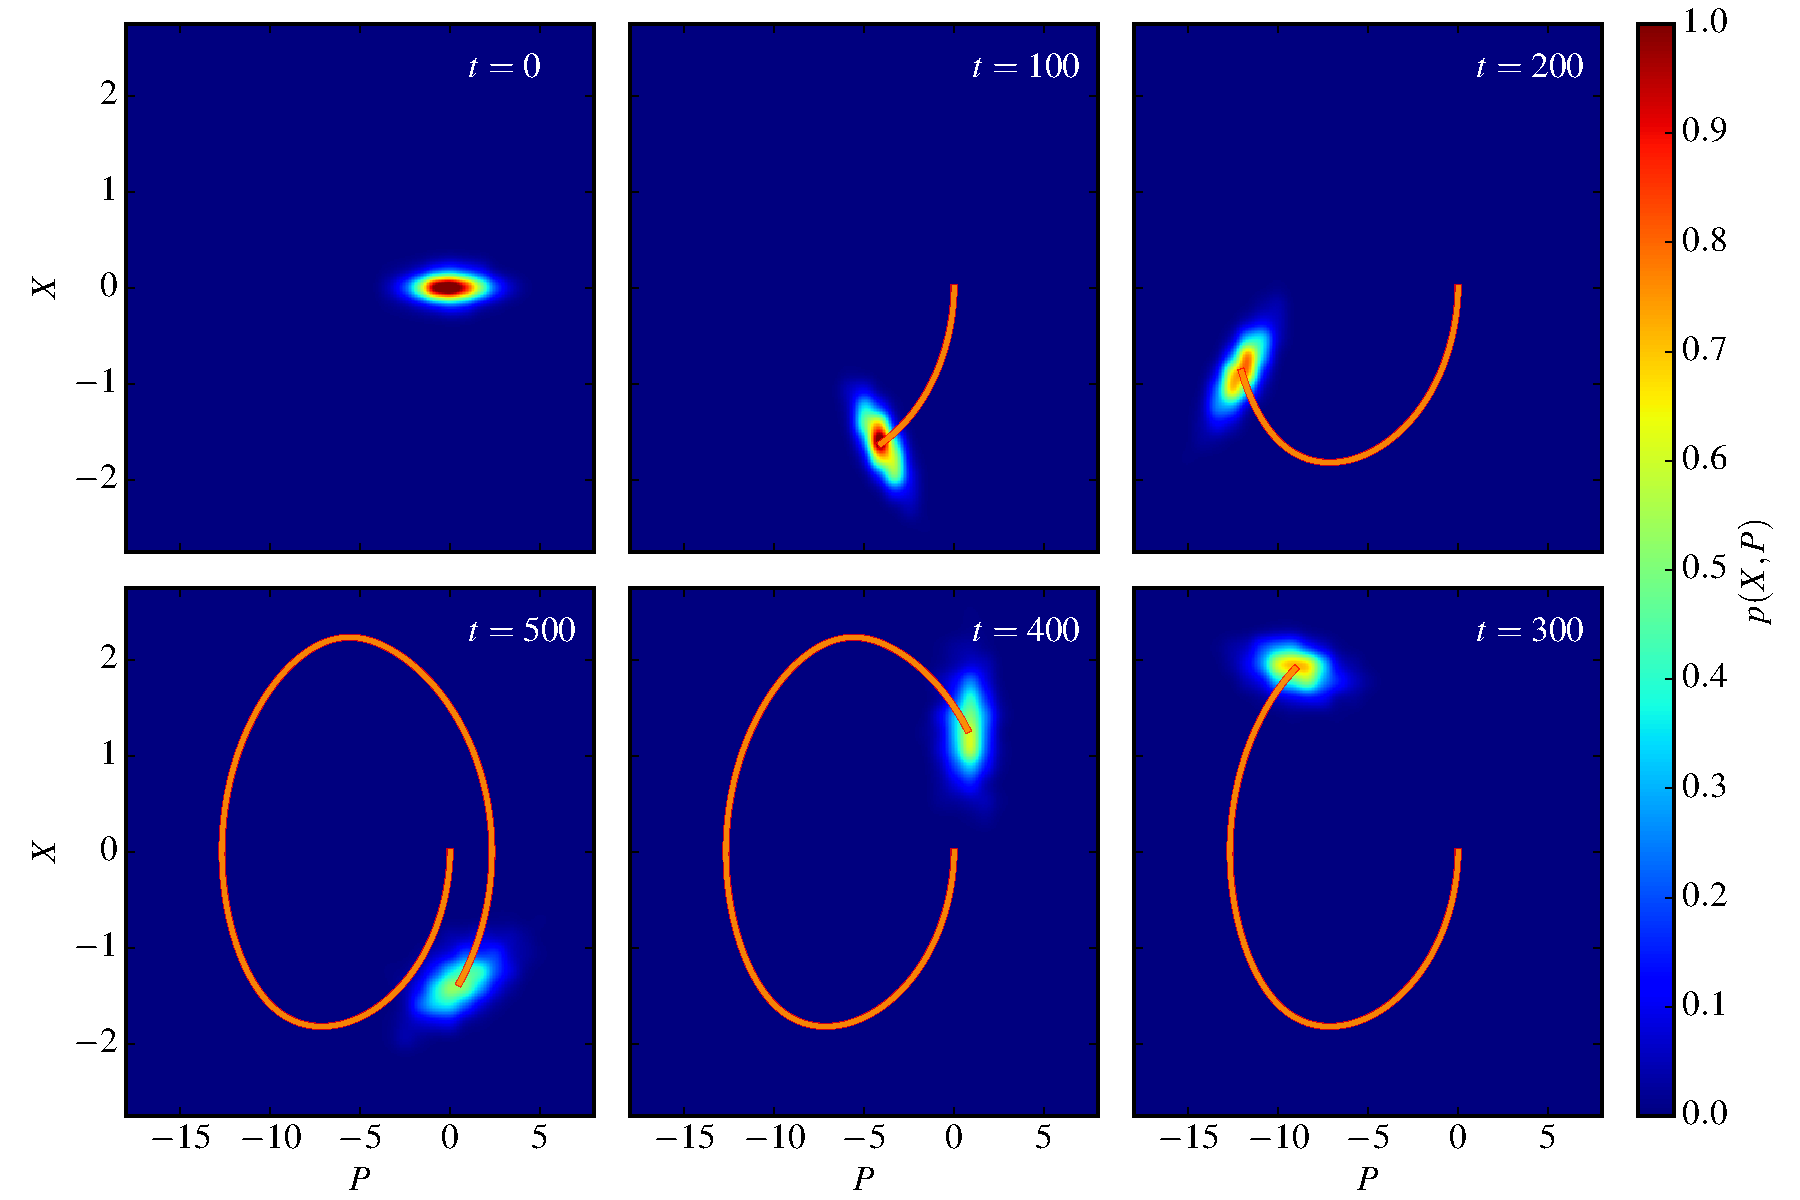
\includegraphics[width=0.9\textwidth]{../report_3/figs/1x3_PDist_Evo_site0.pdf}
	\caption{Time-evolution of vibrational phase-space probability density at the bond between sites 1 and 2 for $\mathbb{M}=1\times 3$. }\label{fig:TD_PSdensity}
\end{figure}
\section{Holstein model}
In the following, we investigate the differences between the model considered before and the Holstein model.
\subsection{Single-dot Holstein model}
The main point is that in the asymetrically coupled Holstein model $g_\uparrow =-g_\downarrow$, the equilibrium position of the phonon mode is $X=P=0$ for all voltages. Therefore, averaging over Boltzmann distribution leads to a steady-state.


%\subsection{Reduction of saturation current}
%As can be seen in \cref{fig:Current_convergence}, the average current slightly oscillates with time. To capture this oscillation, \cref{fig:IV_1x3_MF-HEOM} shows the maximum (red line), minimum (blue line) and average (black line) of the current in the time interval $[200,2000]t_0^{-1}$.
%\begin{figure}[!h]
%	\centering
%	\includegraphics[width=0.95\textwidth]{figs/Currents_1x3_Ehrenfest_P0.5_IV_min_max_mean.pdf}
%	\caption{}\label{fig:IV_1x3_MF-HEOM}
%\end{figure} 
%\subsubsection{Holstein model}
%We consider now a Holstein model with the Hamiltonian
%\begin{equation}
%	H = \varepsilon_0 d^\dagger d + g d^\dagger d X(t) + \sum_{\ell,k} \nu_{\ell,k}d^\dagger d_{\ell k}c + \mathrm{h.c.} + \sum_{\ell,k} \varepsilon_{\ell k}c^\dagger_{\ell k}c^\pdagger_{\ell k}.
%\end{equation}
%Using the unoccupied and occupied dot states as the basis, 
%under the Born-Markov approximation, an equation of motion for the reduced density matrix can be derived. Neglecting further the time-dependence of the system Green functions, the Master equation reads
%\begin{equation}
%	\dot{\rho}(t) = -i[H(t),\rho] + (-\Gamma_L \rho_{00}+\Gamma_R\rho_{11})\vert 0\rangle\langle 0\vert + (\Gamma_L \rho_{00}-\Gamma_R\rho_{11})\vert 1\rangle\langle 1\vert.
%\end{equation}
%Together with the classical equation of motion, the coupled system of equations of motion read
%\begin{align}
%	\dot{\rho}_{00} &= -\Gamma_L\rho_{00}+\Gamma_R\rho_{11}\\
%	\dot{\rho}_{11} &= \Gamma_L\rho_{00}-\Gamma_R\rho_{11}\\
%	\dot{\rho}_{01} &= i\rho_{01}(\varepsilon_0 + gX(t))\\
%	\dot{X} &= \omega_0 P(t)\\
%	\dot{P} &= -g(\rho_{01}(t)+\rho_{11}(t)) - \omega_0^2 X(t).
%\end{align}
%\begin{itemize}
%	\item For single phonon, e.g. on site 2 of a three-dot system, there exists a steady-state current
%	\item Already when placing two phonons, steady-state does not exist.
%\end{itemize}
%\subsection{Floquet-Liouvillian analysis}
%The vibrational dynamics is nearly periodic, such that
%\begin{equation}
%	\mathcal{L}(t) \approx \mathcal{L}(t+\tau)
%\end{equation}
%approximately holds. The time-dependence of the Liouvillian stems from the time-dependence of the classical vibrational modes, which is assumed to have the form given in \cref{eq:AnalyticalVib1,eq:AnalyticalVib2}.
%\subsection{Time-dependent Populations}
%Show that populations are also not stationary for long times, but switch depending on the positions of the phonons.
%Show $(t,V)$ imshow of population on a single site.
%Show $(t,\mathrm{site})$ imshow of all populations on all sites for different times.
%Can be explained with spectrum which is now time-dependent under the influence of phonons.
%Quantization of vibrational motion. Show FFT of population dynamics. Relation to phonon-frequencies. If matching, then there are quanta of vibration exchanged between electrons and vibrations.
%%\subsection{Show that steady-state density matrix is the one of the effective }
%%Clear from the analytical result without the phonons.
%\subsection{Picture 1: Time-dependent spectrum}
%Berry phase effects? 
%\subsection{Picture 2: Transistions induced by el-ph coupling between stationary eigenstates}


\section{Holstein Model}
\subsection{Hamiltonian}
The Hamiltonian of the Holstein model reads
\begin{equation}
	H_\mathrm{Holstein} = \sum_{j\sigma}( \varepsilon_{j\sigma}^\pdagger + g_{j\sigma}^\pdagger [a_j^\dagger+ a_j^\pdagger]) c_{j\sigma}^\dagger c_{j\sigma}^\pdagger - t \sum_{j\sigma}(c_{j\sigma}^\dagger c_{j+1\sigma}^\pdagger  + \mathrm{h.c.}) + \sum_j \omega_j^\pdagger  a_j^\dagger a_j^\pdagger
\end{equation}
consisting of spin-$1/2$ electrons on a lattice, electrons on each level of a site coupling locally to a vibrational mode. We say the electron-phonon coupling is symmetric if $g_{j\sigma}=g_{j\bar{\sigma}}$ and anti-symmetric if $g_{j\sigma}=-g_{j\bar{\sigma}}$. Within the quantum-classical approximation the term $a_j^\dagger+ a_j^\pdagger \rightarrow \sqrt{2\omega_0} X_j$ gets replaced by the classical position $X_j$ and $a_j^\dagger a_j^\pdagger \rightarrow \frac{1}{2}(\omega_jX_j^2+P_j^2)$.
\subsection{Single dot}
Parameters: $\varepsilon_\uparrow = 0.2 = -\varepsilon_\downarrow$, $g_\uparrow = 0.1 = -g_\downarrow$, $\omega_0 = 0.1$, $\Gamma_0 = \frac{1}{4}$ and $\beta = 40$. \Cref{fig:Holstein_1x1_V0.4_multiTraj_current} shows the symmetrized current for 200 trajectories (black lines) and the weighted average (red line) for $V=0.4$. The current relaxes to a steady state. 
\Cref{fig:Holstein_1x1_Pops_currents_phonons_VVar} shows the following averaged quantities for various voltages: (a) Spin-up population, (b) spin-down population, (c) symmetrized current, and (d) phase-space trajectory of the vibrational mode. 
The presented data suggests that a unique steady state exists for all voltages. The time-scale on which this steady-state is reached, however, depends on $V$. For example, for $V=0.4$ the steady state is reached already for $t\sim 3\times 10^3 \Gamma_0^{-1}$, but for $V=2.0$ the steady-state is not reached on the time-scale investigated here.
\begin{figure}[!h]
	\centering
	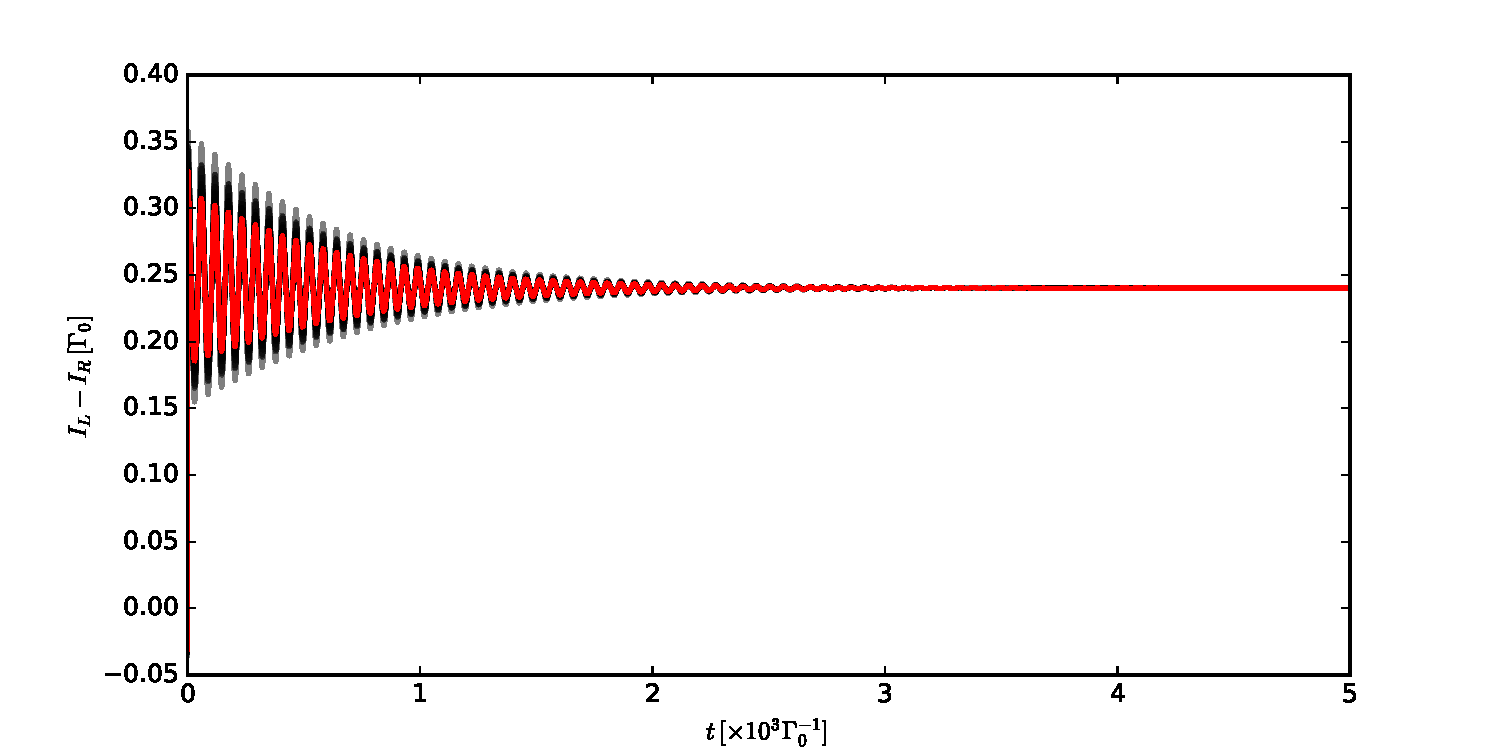
\includegraphics[width=1.0\textwidth]{figs/Holstein_1x1_current_V0.4_multiTraj.pdf}
	\caption{Symmetrized current in the single-dot Holstein model with asymmetric coupling $g = 0.1$ for $V=0.4$. Black lines: Individual trajectories with initial condition sampled from thermal Wigner distribution ($n=200$). Red line: Weighted average.}\label{fig:Holstein_1x1_V0.4_multiTraj_current}
\end{figure}\newpage
\begin{figure}[!h]
	\centering
	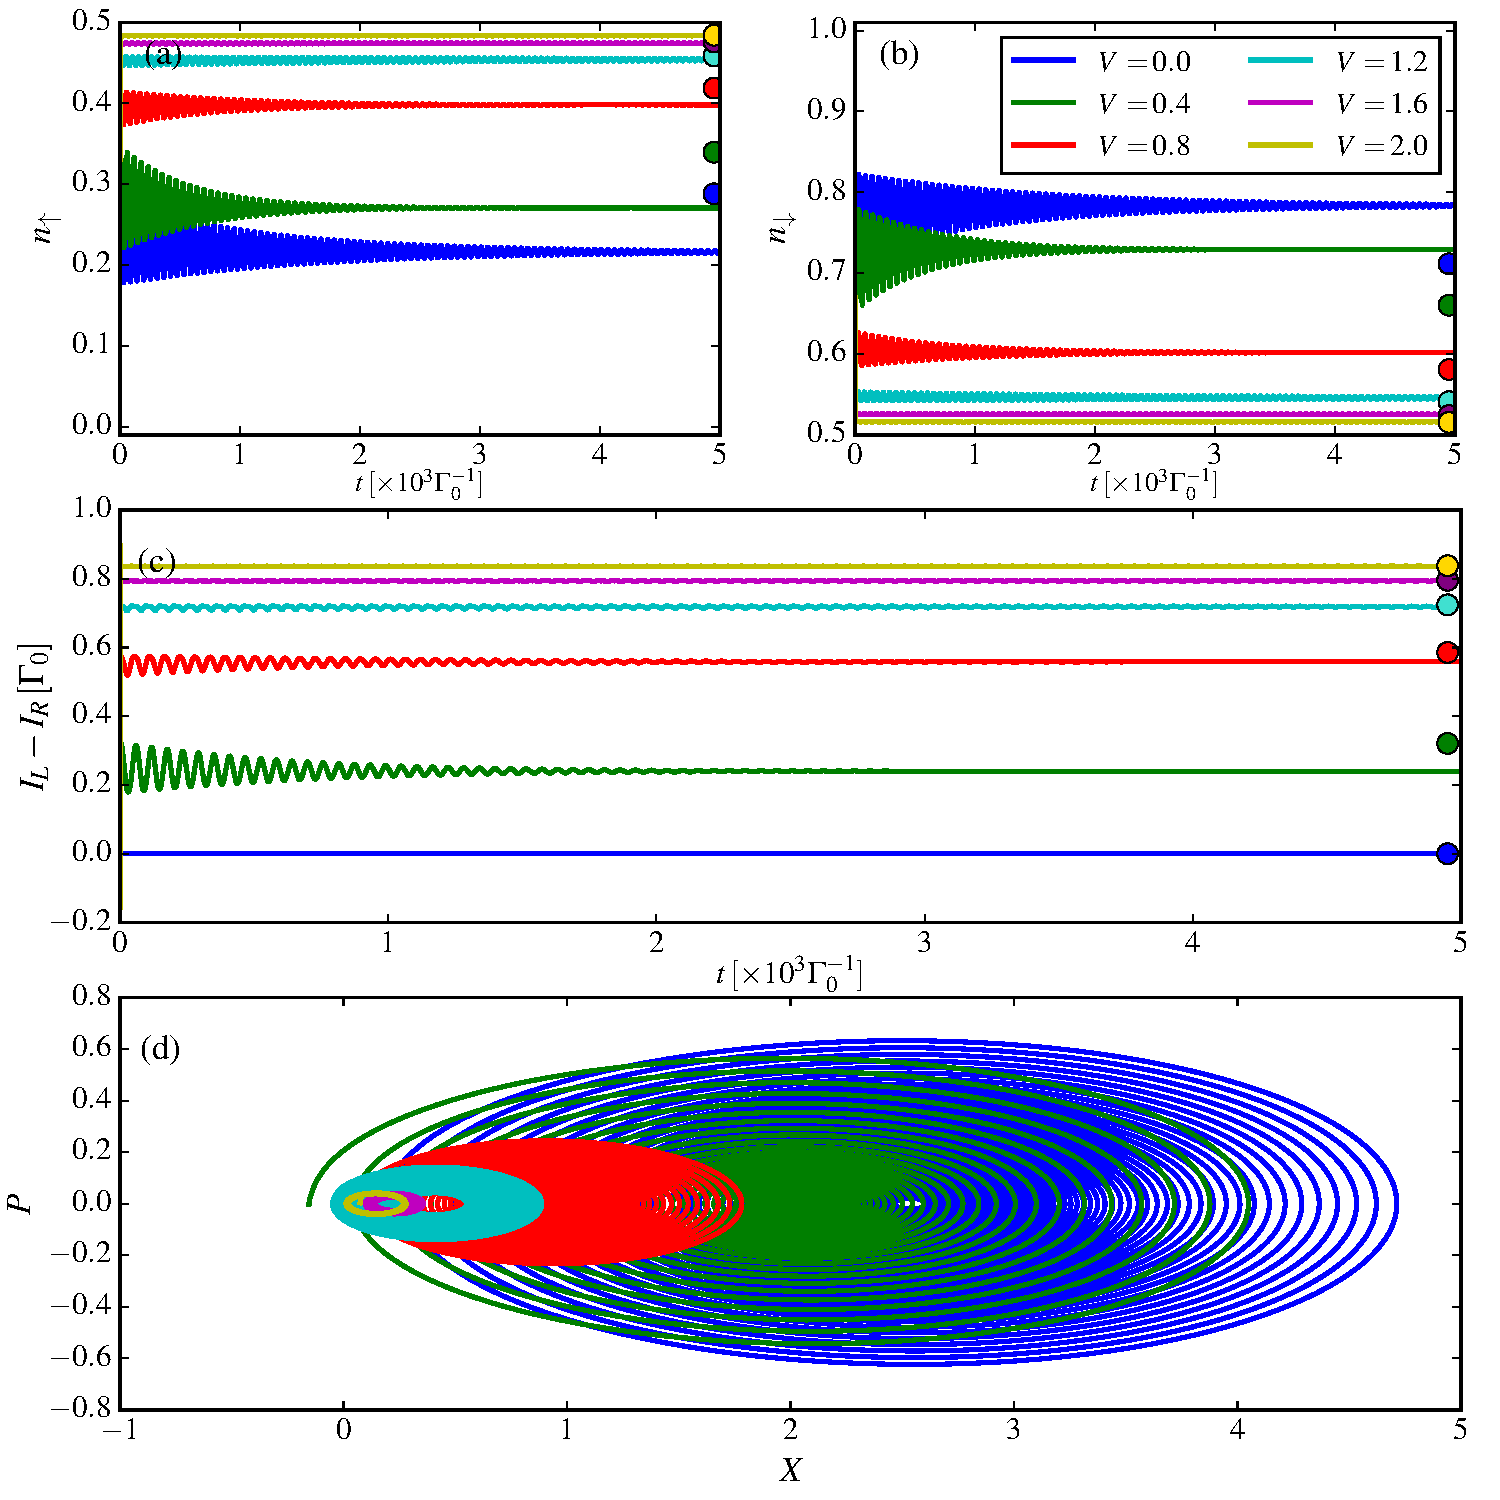
\includegraphics[width=1.0\textwidth]{figs/Pops_currents_phonons_1x1_VVar.pdf}
	\caption{Time-dependence of (a) spin-up population, (b) spin-down population, (c) symmetrized current, and (d) averaged phase-space trajectories in the single Holstein dot with asymmetric coupling. Different lines denote different voltages $V$. Full circles in (a)-(c) show the steady-state values for $g=0$. For all voltages, the sample size is $n=200$.}\label{fig:Holstein_1x1_Pops_currents_phonons_VVar}
\end{figure}\newpage
\begin{figure}[!h]
	\centering
	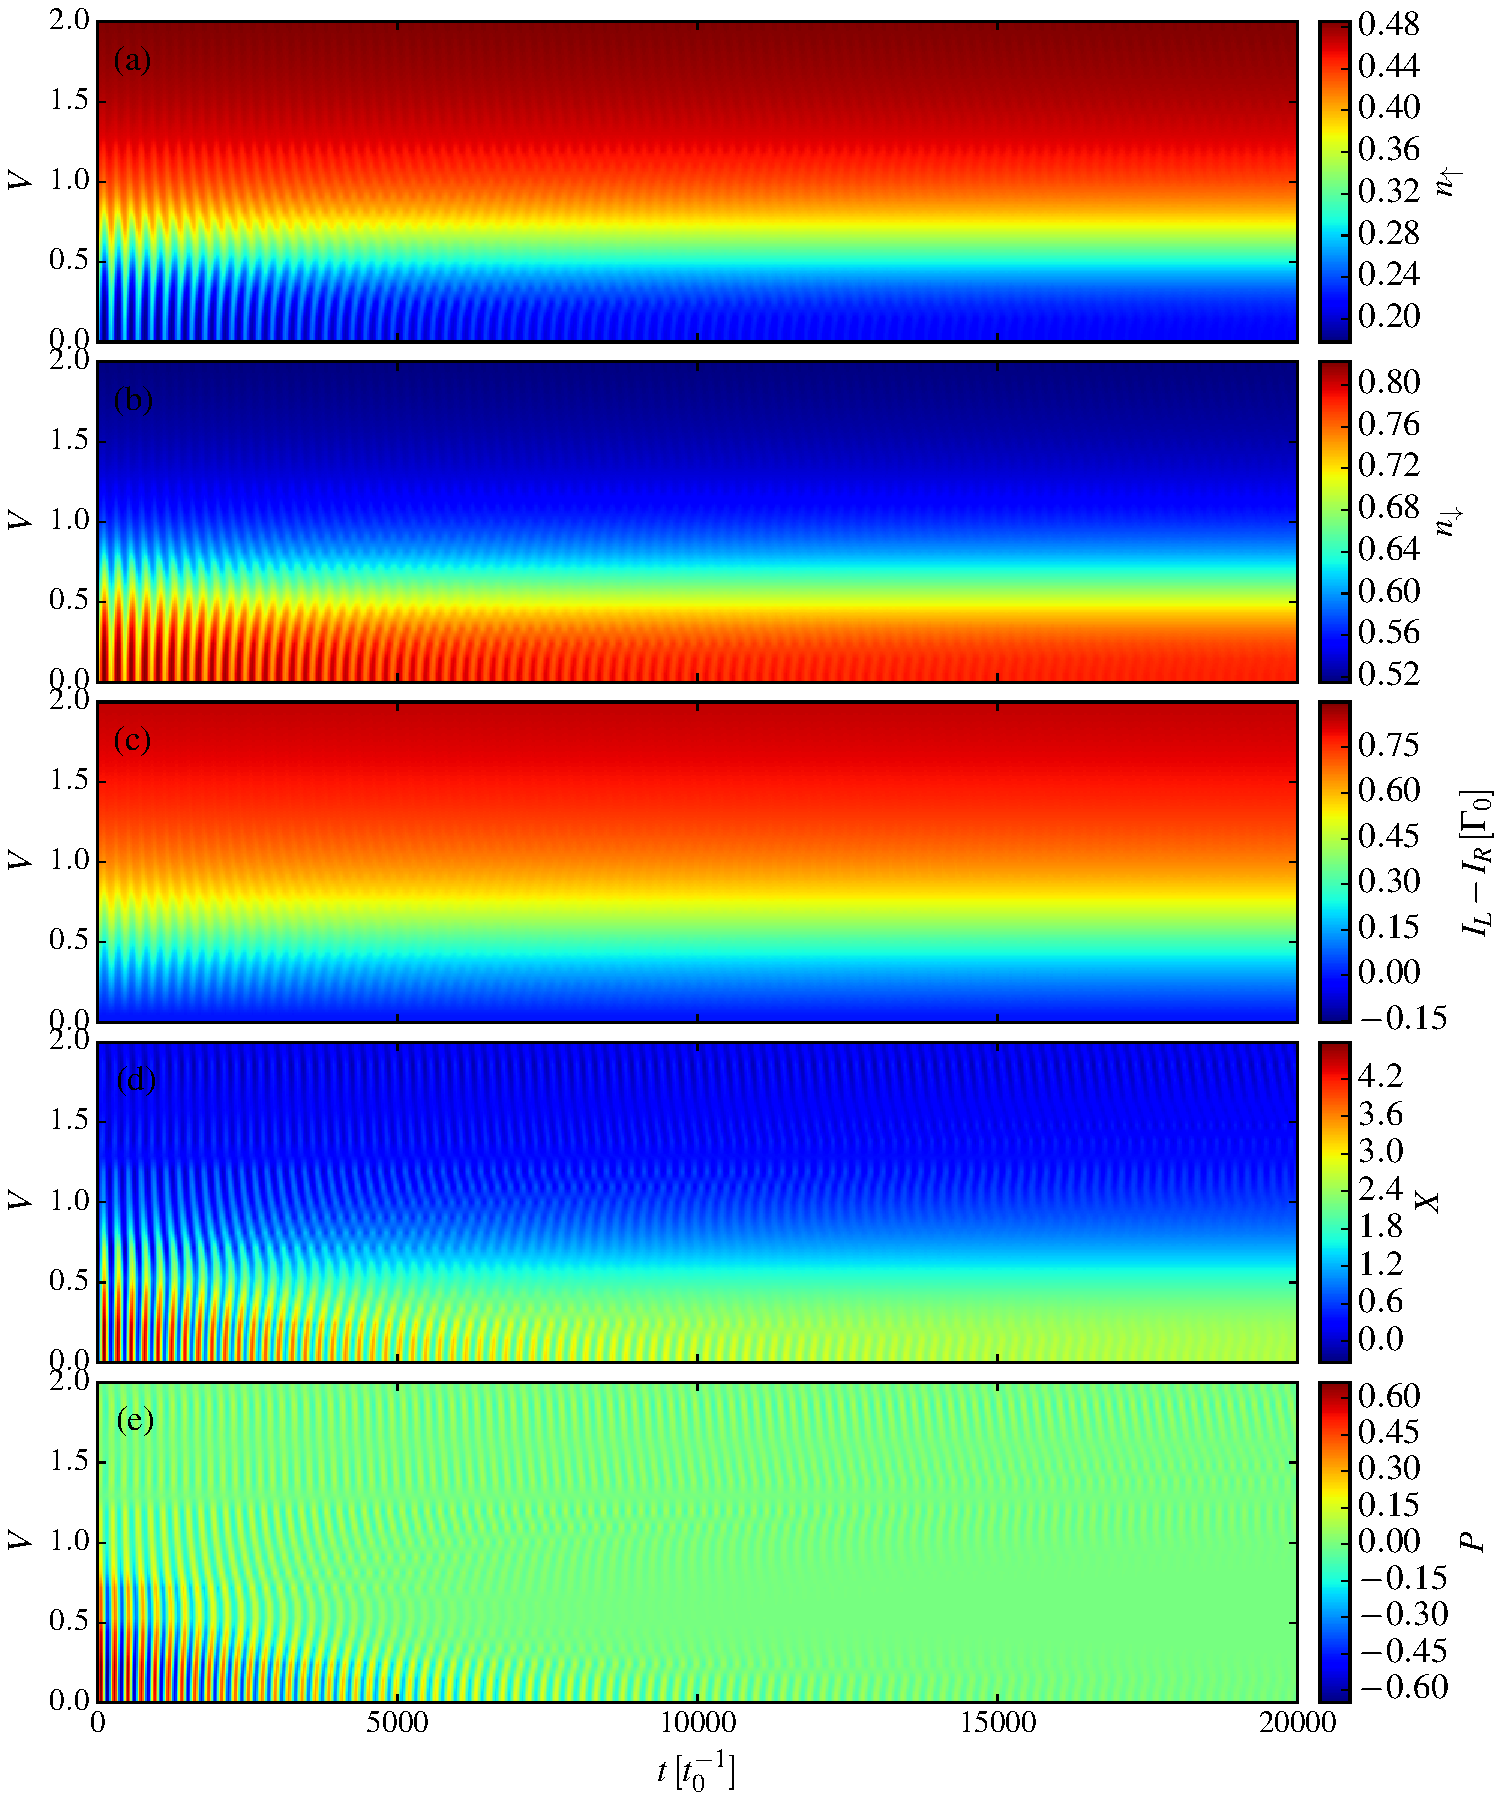
\includegraphics[width=1.0\textwidth]{figs/Pops_currents_phonons_imshow_1x1_VVar.pdf}
	\caption{Voltage dependence of dynamics of (a) spin-up population, (b) spin-down population, (c) symmetrized current, (d) vibrational position and (e) momentum. Parameters are given in the main text.}
\end{figure}\newpage
\begin{figure}[!h]
	\centering
	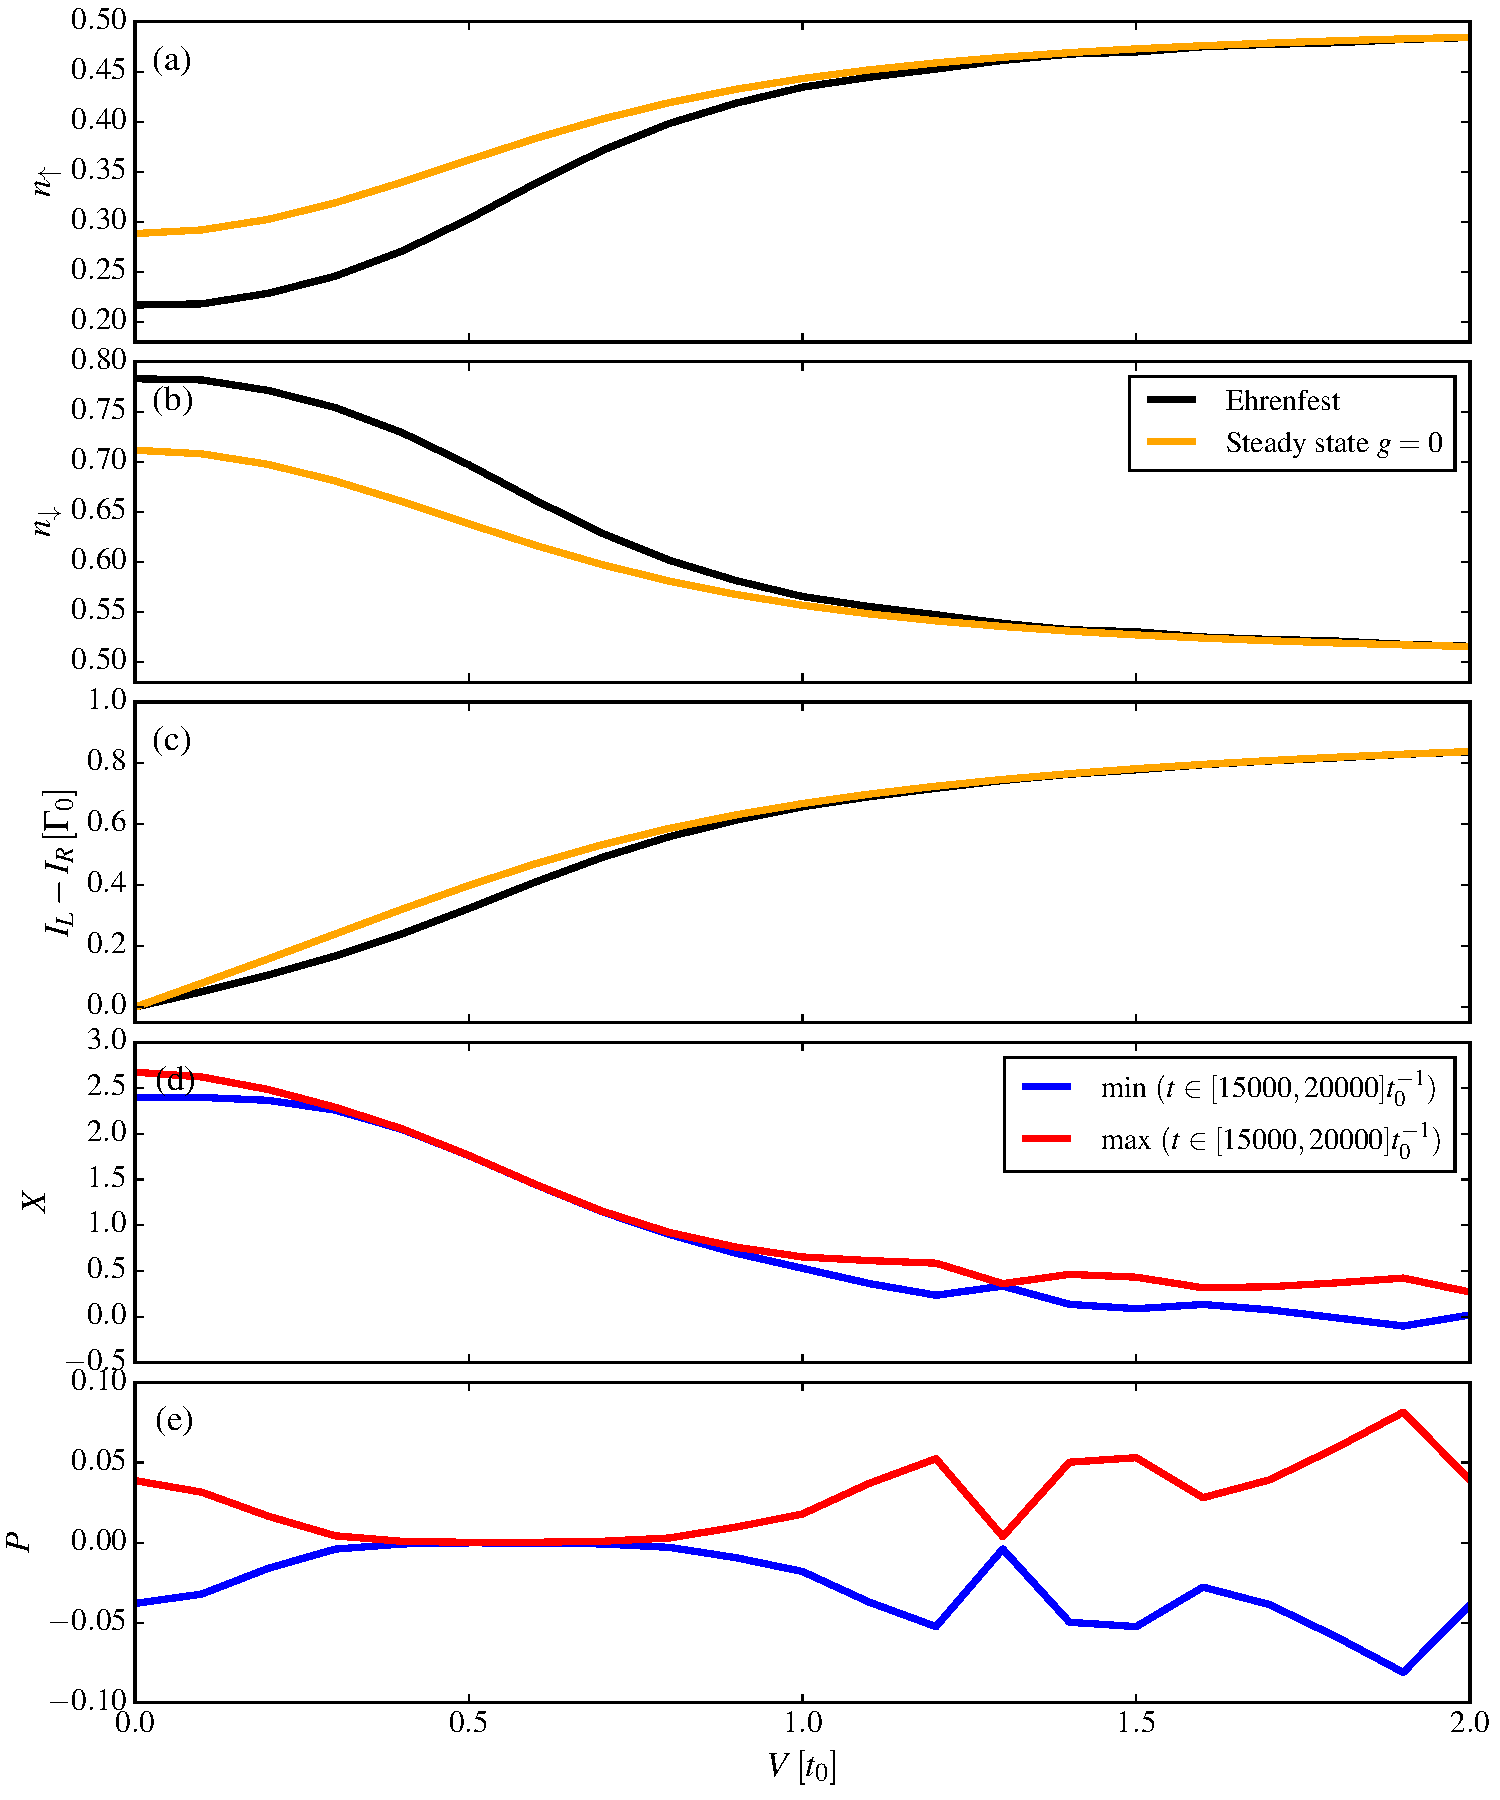
\includegraphics[width=1.0\textwidth]{figs/Pops_currents_phonons_steadyState_1x1_VVar.pdf}
	\caption{Steady-state values. Black lines denote the Ehrenfest calculation with $g=0.1$, orange lines calculations with $g=0$. Red lines are the maximal value of $X,P$ and blue lines the minimum within the interval $[15000,20000]t_0^{-1}$.}
\end{figure}\newpage
\section{Peierls Model}
\subsection{Model}
The Hamiltonian of the Peierls model reads
\begin{equation}
	H_\mathrm{Peierls} = \sum_{j\sigma} \varepsilon_{j\sigma}^\pdagger  c_{j\sigma}^\dagger c_{j\sigma}^\pdagger + \sum_{j\sigma}(-t + g_{j\sigma}^\pdagger [a_j^\dagger+ a_j^\pdagger])(c_{j\sigma}^\dagger c_{j+1\sigma}^\pdagger  + \mathrm{h.c.}) + \sum_j \omega_j^\pdagger  a_j^\dagger a_j^\pdagger
\end{equation}
\subsection{Double dot}
Parameters: $\varepsilon_\uparrow = -\varepsilon_\downarrow =0.2, t_0 = 1, t_1 = 0.1t_0, \omega_0 = 0.1/t_0, \Gamma_0 = t_0/4, \beta = 40$.
\begin{figure}[!h]
	\centering
	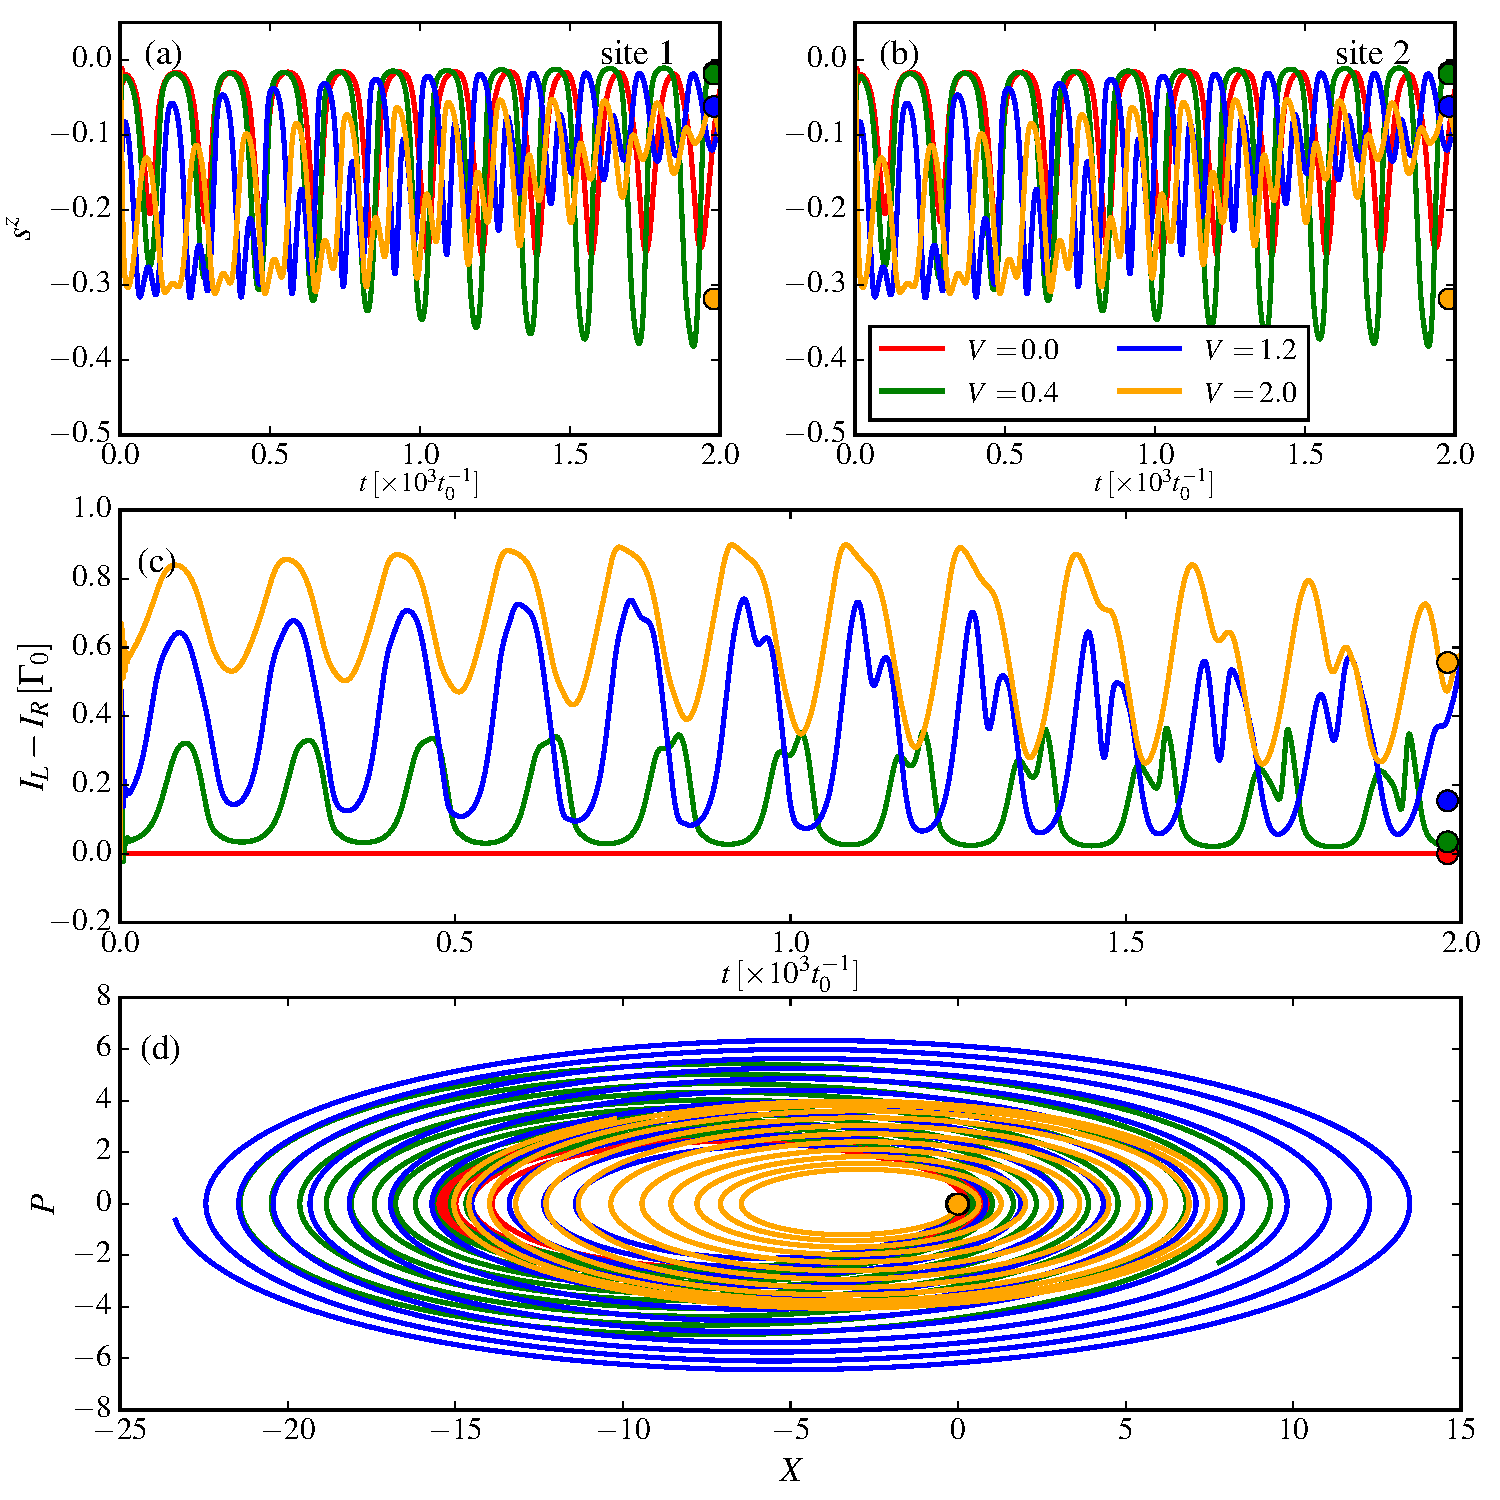
\includegraphics[width=1.0\textwidth]{figs/Pops_currents_phonons_Peierls_1x2_VVar.pdf}
	\caption{Peierls model for $L=2$ and $t_1=0.1$.}
\end{figure}
\begin{figure}[!h]
	\centering
	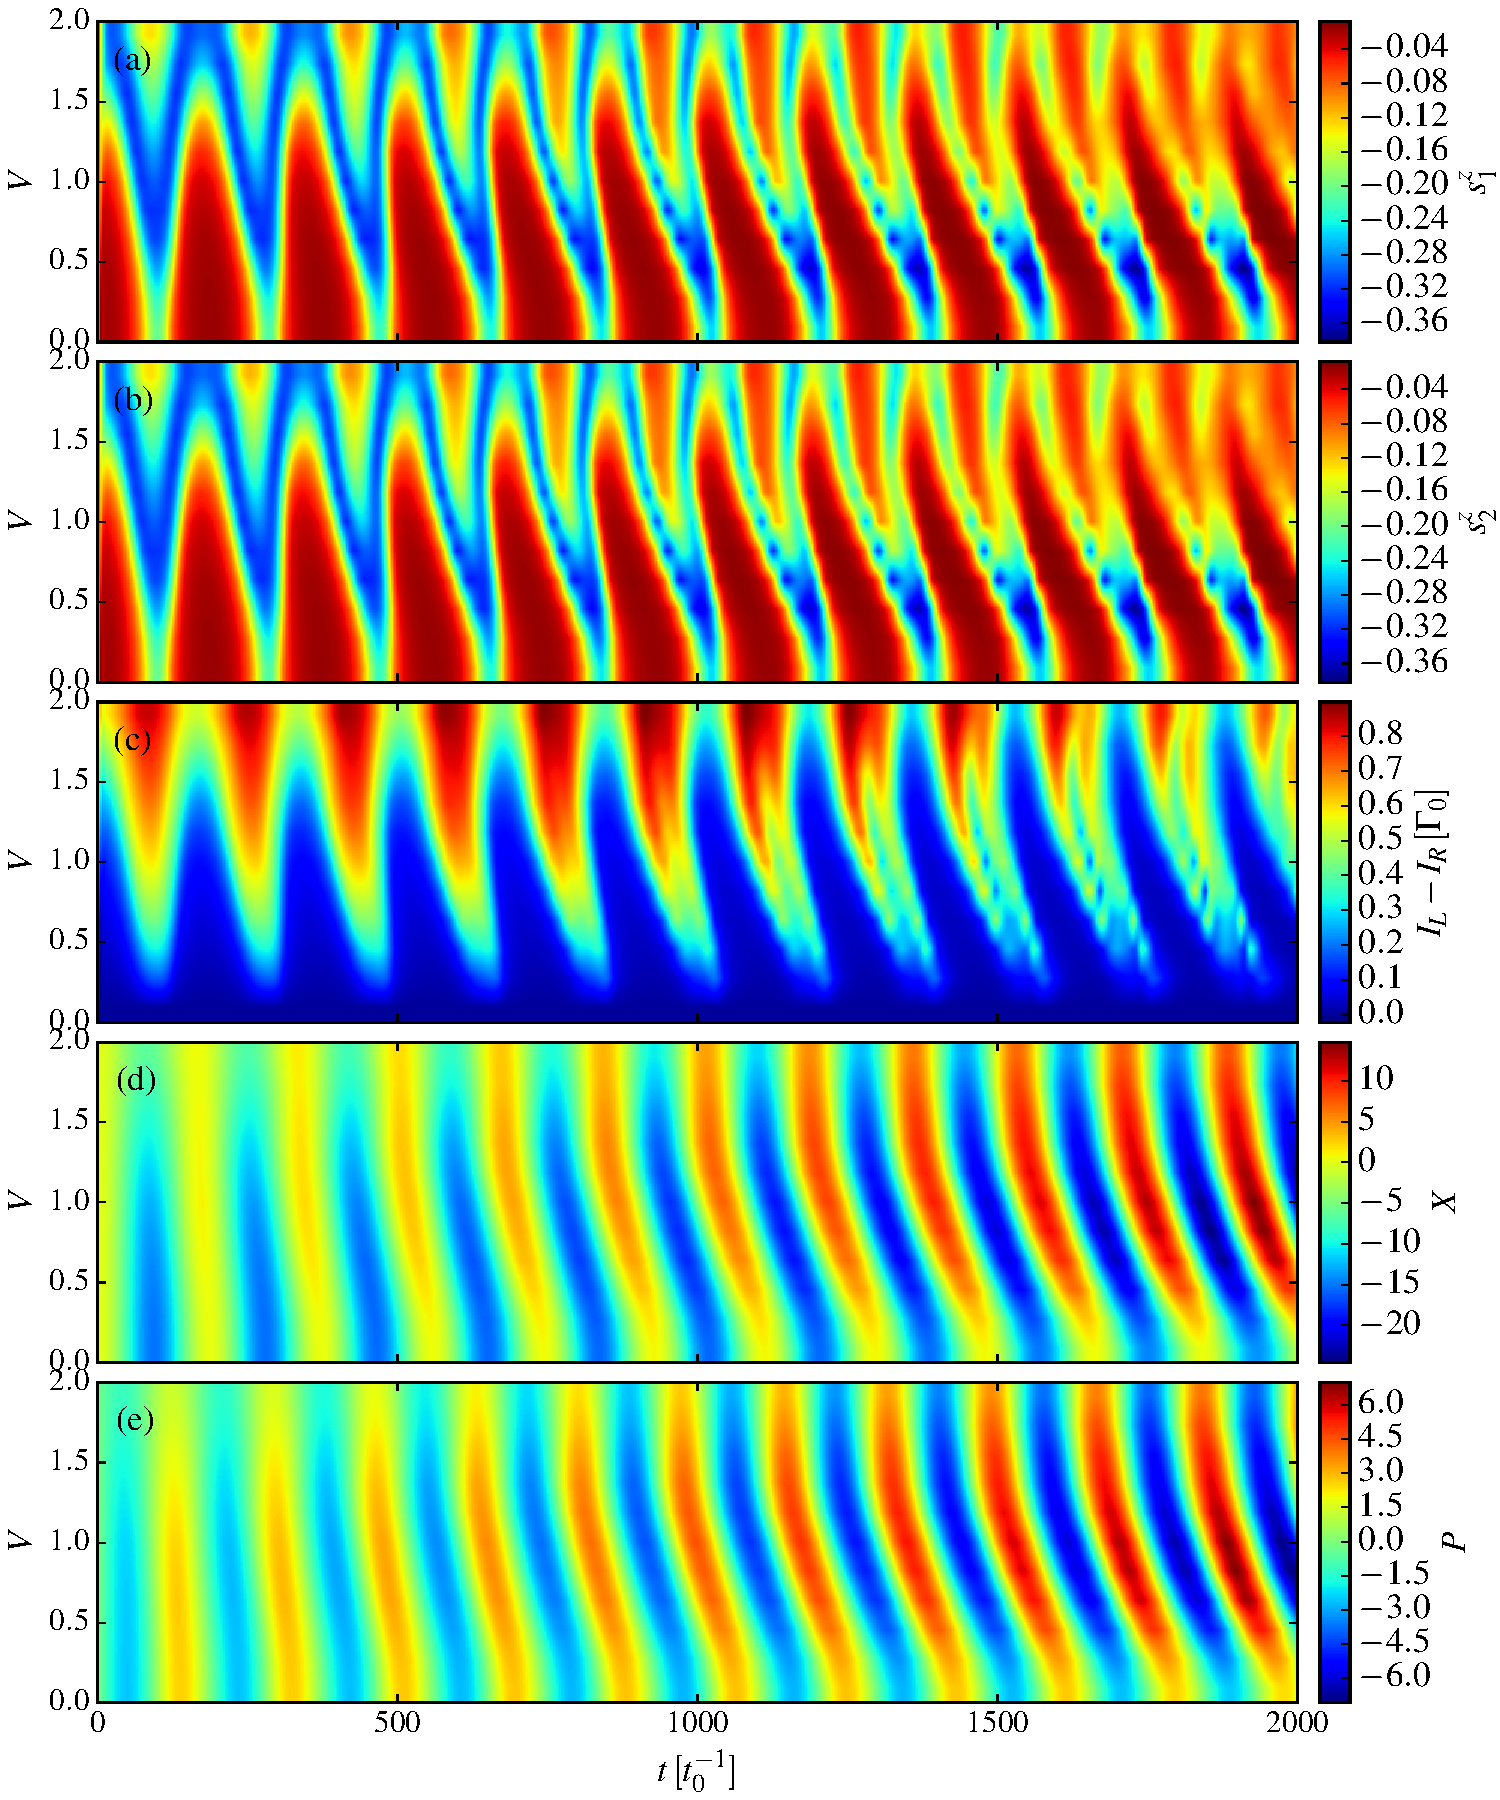
\includegraphics[width=1.0\textwidth]{figs/Pops_currents_phonons_imshow_Peierls_1x2_VVar.pdf}
	\caption{Peierls model.}
\end{figure}
\printbibliography
\end{document}




